\chapter{NLP Applications}
\label{chap6:nlp}

In this chapter, I apply the concept of lifelong representation learning for a wide spectrum of NLP applications.
Natural language processing needs lifelong learning because as a form of human knowledge, texts need to be integrated into the agent for understanding and reasoning for agent's policy.

I will first focus on two (2) tasks in aspect-based sentiment analysis: aspect extraction and aspect sentiment classification.
Then I switch to a novel task in my earlier years of PhD study: complementary entity recognition, which aims to identify multiple entities and their relations.
Then I switch to review-based question answering. Reading comprehension is an important task in question answering because its good usage of human writen texts for answers. I will propose some novel review-based QA tasks, with results indicating the importance of lifelong representation.
Lastly, I will switch to the dialog system.
I will first talk about the conversational version of QA and then switch to a novel type of dialog system: conversational recommendation, which leverages lifelong graph representation learning for reasoning dialog policy.

\section{Sentiment Analysis}
\label{chap6:sec:sa}

Sentiment analysis aims to detect people's polarity from opinion text such as reviews and tweets \cite{Liu2012}.
More specifically, aspect-based sentiment analysis (ABSA) focuses in fine-grained sentiment analysis over aspects and possibly their categories.
ABSA aims to detect the aspects $a$ in opinion texts and their associated polarities $(a, p)$s.
This naturally has two sub-tasks in ABSA: \underline{aspect extraction} and \underline{aspect sentiment classification}.

\subsection{-- Aspect Extraction}

%One key task of fine-grained sentiment analysis of product reviews is to extract product aspects or features that users have expressed opinions on. This paper focuses on supervised aspect extraction using deep learning. Unlike other highly sophisticated supervised deep learning models, this paper proposes a novel and yet simple CNN model employing two types of pre-trained embeddings for aspect extraction: general-purpose embeddings and domain-specific embeddings. Without using any additional supervision, this model achieves surprisingly good results, outperforming state-of-the-art sophisticated existing methods. To our knowledge, this paper is the first to report such a double embeddings based CNN model for aspect extraction and achieve very good results. 

%\section{Introduction}
Aspect extraction is an important task in sentiment analysis \cite{HuL2004} and has many applications to its downstream tasks\cite{Liu2012}.
It aims to extract opinion targets (or aspects) from opinion text. 
In product reviews, aspects are product attributes or features. 
For example, from ``\textit{Its speed is incredible}'' in a laptop review, it aims to extract ``speed''. 

Aspect extraction has been performed using supervised \cite{Jakob2010,chernyshevich2014ihs,shu2017lifelong} and unsupervised approaches \cite{HuL2004,ZhuangJZ2006,MeiLWSZ2007,QiuLBC2011,yin2016unsupervised,he2017unsupervised}. 
Recently, supervised deep learning models achieved state-of-the-art performances \cite{li2017deep}. Many of these models use handcrafted features, lexicons, and complicated neural network architectures \cite{poria2016aspect,wang2016recursive,wang2017coupled,li2017deep}. 
Although these approaches can achieve better performances than their prior works, two other considerations are also important.
(1) Automated feature (representation) learning is always preferred. 
How to achieve competitive performances without manually crafting features is an important question. 
(2) According to Occam's razor principle \cite{blumer1987occam}, a simple model is always preferred over a complex model.
This is especially important when the model is deployed in a real-life application (e.g., chatbot), where a complex model will slow down the speed of inference. Thus, to achieve competitive performance whereas keeping the model as simple as possible is important. This paper proposes such a model. 

To address the first consideration, we propose a double embeddings mechanism (as discussed in Chapter \ref{chap3:word}) that is shown crucial for aspect extraction.
The embedding layer is the very first layer, where all the information about each word is encoded.
The quality of the embeddings determines how easily later layers (e.g., LSTM, CNN or attention) can decode useful information.
Existing deep learning models for aspect extraction use either a pre-trained general-purpose embedding, e.g., GloVe \cite{pennington2014glove}, or a general review embedding \cite{poria2016aspect}.
However, aspect extraction is a complex task that also requires fine-grained domain embeddings.
For example, in the previous example, detecting ``speed'' may require embeddings of both ``Its'' and ``speed''.
However, the criteria for good embeddings for ``Its'' and ``speed'' can be different.
``Its'' is a general word and the general embedding (trained from a large corpus) is likely to have better representation for ``Its''.
But, ``speed'' has a very fine-grained meaning (e.g., how many instructions per second) in the \textit{laptop} domain, whereas ``speed'' in general embeddings or general review embeddings may mean how many miles per second.
So using in-domain embeddings is important even when the in-domain embedding corpus is not large. 
Thus, we leverage both general embeddings and domain embeddings and let the rest of the network to decide which embeddings have more useful information.

To address the second consideration, we use a pure Convolutional Neural Network (CNN) \cite{lecun1995convolutional} model for sequence labeling.
Although most existing models use LSTM \cite{hochreiter1997long} as the core building block to model sequences \cite{liu2015fine,li2017deep}, we noticed that CNN is also successful in many NLP tasks \cite{kim2014convolutional,zhang2015character,gehring2017convolutional}.
One major drawback of LSTM is that LSTM cells are sequentially dependent.
The forward pass and backpropagation must serially go through the whole sequence, which slows down the training/testing process
\footnote{We notice that a GPU with more cores has no training time gain on a low-dimensional LSTM because extra cores are idle and waiting for the other cores to sequentially compute cells.}.
One challenge of applying CNN on sequence labeling is that convolution and max-pooling operations are usually used for summarizing sequential inputs and the outputs are not well-aligned with the inputs. %We discuss the solutions in Section \ref{chap3:sec:model}.
We call the proposed model \underline{D}ual \underline{E}mbeddings \underline{CNN} (DE-CNN).
To the best of our knowledge, this is the first paper that reports a double embedding mechanism and a pure CNN-based sequence labeling model for aspect extraction.

\textbf{Related Work}

Sentiment analysis has been studied at document, sentence and aspect levels \cite{Liu2012,Pang2008OMS,Cambria2012}. This work focuses on the aspect level \cite{HuL2004}. Aspect extraction is one of its key tasks and has been performed using both unsupervised and supervised approaches. 
The unsupervised approach includes methods such as frequent pattern mining \cite{HuL2004,PopescuNE2005}, syntactic rules-based extraction \cite{ZhuangJZ2006,WangBo2008,QiuLBC2011}, topic modeling \cite{MeiLWSZ2007,TitovM2008,Lin2009,Moghaddam2011}, word alignment \cite{KangLiu2013IJCAI} and label propagation \cite{Zhou-wan-xiao:2013:EMNLP,shu2016lifelong}.

Traditionally, the supervised approach \cite{Jakob2010,Mitchell-EtAl:2013:EMNLP,shu2017lifelong} uses Conditional Random Fields (CRF) \cite{Lafferty2001conditional}.
Recently, deep neural networks are applied to learn better features for supervised aspect extraction, e.g., using
LSTM \cite{williams1989learning,hochreiter1997long,liu2015fine} and
attention mechanism \cite{wang2017coupled,he2017unsupervised} together with manual features \cite{poria2016aspect,wang2016recursive}.
Further, \cite{wang2016recursive,wang2017coupled,li2017deep} also proposed aspect and opinion terms co-extraction via a deep network.
They took advantage of the gold-standard opinion terms or sentiment lexicon for aspect extraction.
The proposed approach is close to \cite{liu2015fine}, where only the annotated data for aspect extraction is used. 
However, we will show that our approach is more effective even compared with baselines using additional supervision and/or resources.

The proposed embedding mechanism is related to cross domain embeddings \cite{bollegala2015unsupervised,bollegala2017think} and domain-specific embeddings \cite{xumeta,Xu2018pro}. 
However, we require the domain of the domain embeddings must exactly match the domain of the aspect extraction task. 
CNN \cite{lecun1995convolutional,kim2014convolutional} is recently adopted for named entity recognition \cite{strubell2017fast}.
CNN classifiers are also used in sentiment analysis \cite{poria2016aspect,chen2017improving}.
We adopt CNN for sequence labeling for aspect extraction because CNN is simple and parallelized.

\textbf{Double Embedding for Sequence Labeling}

Following the idea of fusion general and domain-specific embeddings in \ref{chap3:word}, we have the following CNN-based model for aspect extraction.
%As a counter-example, if the training/testing data is in the \textit{laptop} domain, then embeddings from the \textit{electronics} domain are considered to be out-of-domain embeddings (e.g., the word ``adapter'' may represent different types of adapters in \textit{electronics} rather than exactly a \textit{laptop} adapter). That is, only laptop reviews are considered to be in domain. 

The proposed model is depicted in \ref{chap6:fig:fr}.
It has 2 embedding layers, 4 CNN layers, a fully-connected layer shared across all positions of words, and a softmax layer over the labeling space $\mathcal{Y}=\{B, I, O\}$ for each position of inputs.
Note that an aspect can be a phrase and $B$, $I$ indicate the beginning word and non-beginning word of an aspect phrase and $O$ indicates non-aspect words.

\begin{figure}[H]
\centering    
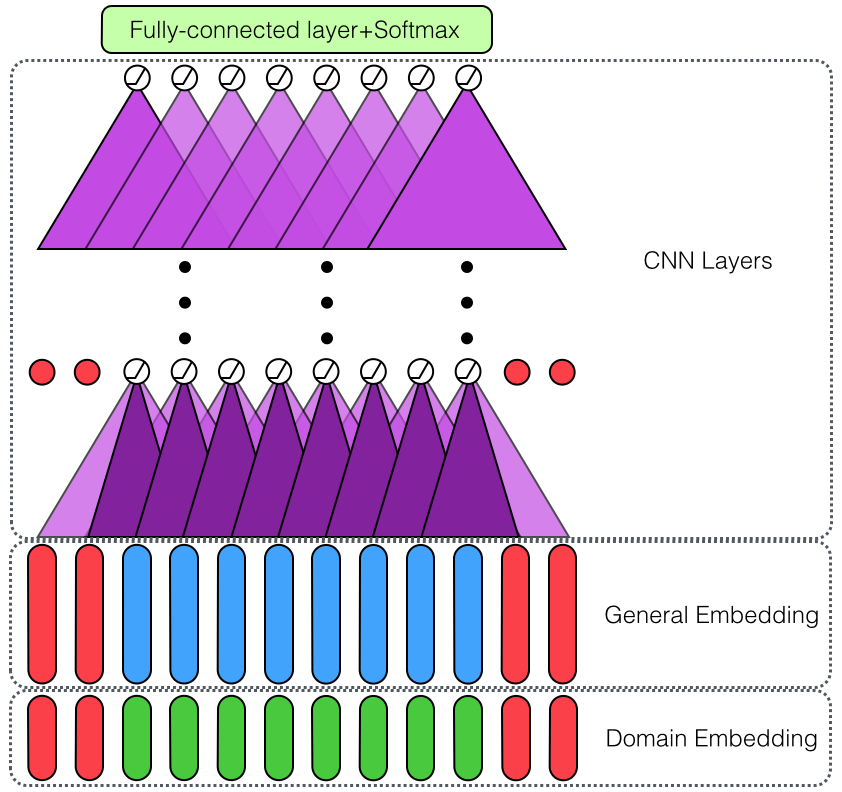
\includegraphics[width=5.in]{fig/acl18_fig.png}
    \caption{DE-CNN}
    \label{chap6:fig:fr}
\end{figure}

After leveraging the double embedding layers discussed in Chapter \ref{chap3:sec:double}, we apply CNN layers for building representations for aspect extraction.
A CNN layer has many 1D-convolution filters and each (the $r$-th) filter has a fixed kernel size $k=2c+1$ and performs the following convolution operation and ReLU activation: 
%\vspace{-0.5cm}
\begin{equation}
x_{i,r}^{(l+1)}=\max\bigg(0, (\sum_{j=-c}^c w_{j,r}^{(l)} x_{i+j}^{(l)})+b_r^{(l)}\bigg),
\end{equation}
%\vspace{-0.3cm}
%\noindent
where $l$ indicates the $l$-th CNN layer. 
We apply each filter to all positions $i=1:n$.
So each filter computes the representation for the $i$-th word along with $2c$ nearby words in its context.  
Note that we force the kernel size $k$ to be an odd number and set the stride step to be 1 and further pad the left $c$ and right $c$ positions with all zeros.  
In this way, the output of each layer is well-aligned with the original input $\mathbf{x}$ for sequence labeling purposes.
For the first ($l=1$) CNN layer, we employ two different filter sizes. 
For the rest 3 CNN ($l \in \{2, 3, 4\}$) layers, we only use one filter size.
We will discuss the details of the hyper-parameters in the experiment section.
Finally, we apply a fully-connected layer with weights shared across all positions and a softmax layer to compute label distribution for each word.
The output size of the fully-connected layer is $|\mathcal{Y}|=3$.
We apply dropout after the embedding layer and each ReLU activation.
Note that we do not apply any max-pooling layer after convolution layers because a sequence labeling model needs good representations for every position and max-pooling operation mixes the representations of different positions, which is undesirable (we show a max-pooling baseline in the experiments).

We further conduct BERT model for aspect extraction. We omit the details of BERT for aspect extraction as it is already discussed in Chapter \ref{chap4:context}.

\textbf{Experiments}

\begin{table}
    \label{tab:dataset} 
    \centering
    \scalebox{0.8}{
        \begin{tabular}{c|c|c}
        \hline
            {\bf Description}  &{\bf Training }        &{\bf Testing }  \\
                               &{\bf \#S./\#A.} &{\bf \#S./\#A.}  \\\hline
            SemEval-14 Laptop  &3045/2358              &800/654\\\hline
            SemEval-16 Restaurant&2000/1743            &676/622\\\hline
        \end{tabular}
    }
    \caption{Dataset for AE}
\end{table}

Following the experiments of a recent aspect extraction paper \cite{li2017deep},
we conduct experiments on two benchmark datasets from SemEval challenges \cite{pontiki2014SemEval,pontiki2016semeval} as shown in Table \ref{tab:dataset}. 
The first dataset is from the \textit{laptop} domain on subtask 1 of SemEval-2014 Task 4.
The second dataset is from the \textit{restaurant} domain on subtask 1 (slot 2) of SemEval-2016 Task 5.
These two datasets consist of review sentences with aspect terms labeled as spans of characters.
We use NLTK\footnote{\url{http://www.nltk.org/} } to tokenize each sentence into a sequence of words. 

For the general-purpose embeddings, we use the glove.840B.300d embeddings \cite{pennington2014glove}, which are pre-trained from a corpus of 840 billion tokens that cover almost all web pages. These embeddings have 300 dimensions.
For domain-specific embeddings, we collect a laptop review corpus and a restaurant review corpus and use fastText \cite{bojanowski2016enriching} to train domain embeddings.  
The laptop review corpus contains all laptop reviews from the Amazon Review Dataset \cite{he2016ups}.
The restaurant review corpus is from the Yelp Review Dataset Challenge \footnote{\url{https://www.yelp.com/dataset/challenge} }.
We only use reviews from restaurant categories that the second dataset is selected from \footnote{\url{http://www.cs.cmu.edu/~mehrbod/RR/Cuisines.wht} }.
We set the embedding dimensions to 100 and the number of iterations to 30 (for a small embedding corpus, embeddings tend to be under-fitted), and keep the rest hyper-parameters as the defaults in fastText.
We further use fastText to compose out-of-vocabulary word embeddings via subword N-gram embeddings.

\textbf{Baseline Methods for DE-CNN}\\
We perform a comparison of DE-CNN with three groups of baselines using the standard evaluation of the datasets\footnote{\url{http://alt.qcri.org/semeval2014/task4}} \footnote{\url{http://alt.qcri.org/semeval2016/task5}}.
The results of the first two groups are copied from \cite{li2017deep}.
The first group uses single-task approaches.

\textbf{CRF} is conditional random fields with basic features\footnote{\url{http://sklearn-crfsuite.readthedocs.io/en/latest/tutorial.html} } and GloVe word embedding\cite{pennington2014glove}.

\textbf{IHS\_RD} \cite{chernyshevich2014ihs} and \textbf{NLANGP} \cite{toh2016nlangp} are best systems in the original challenges \cite{pontiki2014SemEval,pontiki2016semeval}.

\textbf{WDEmb} \cite{yin2016unsupervised} enhanced CRF with word embeddings, linear context embeddings and dependency path embeddings as input.

\textbf{LSTM} \cite{liu2015fine,li2017deep} is a vanilla BiLSTM.

\textbf{BiLSTM-CNN-CRF} \cite{Reimers:2017:EMNLP} is the state-of-the-art from the Named Entity Recogntion (NER) community. We use this baseline\footnote{\url{https://github.com/UKPLab/emnlp2017-bilstm-cnn-crf} } to demonstrate that a NER model may need further adaptation for aspect extraction.

The second group uses multi-task learning and also take advantage of gold-standard opinion terms/sentiment lexicon.

\textbf{RNCRF} \cite{wang2016recursive} is a joint model with a dependency tree-based recursive neural network and CRF for aspect and opinion terms co-extraction. 
Besides opinion annotations, it also uses handcrafted features.

\textbf{CMLA} \cite{wang2017coupled} is a multi-layer coupled-attention network that also performs aspect and opinion terms co-extraction. It uses gold-standard opinion labels in the training data.

\textbf{MIN} \cite{li2017deep} is a multi-task learning framework that has (1) two LSTMs for jointly extraction of aspects and opinions, and (2) a third LSTM for discriminating sentimental and non-sentimental sentences. 
A sentiment lexicon and high precision dependency rules are employed to find opinion terms. 

The third group is the variations of DE-CNN.

\textbf{GloVe-CNN} only uses glove.840B.300d to show that domain embeddings are important. 

\textbf{Domain-CNN} does not use the general embeddings to show that domain embeddings alone are not good enough as the domain corpus is limited for training good general word embeddings.

\textbf{MaxPool-DE-CNN} adds max-pooling in the last CNN layer. We use this baseline to show that the max-pooling operation used in the traditional CNN architecture is harmful to sequence labeling.

\textbf{DE-OOD-CNN} replaces the domain embeddings with out-of-domain embeddings to show that a large out-of-domain corpus is not a good replacement for a small in-domain corpus for domain embeddings.
We use all \textit{electronics} reviews as the out-of-domain corpus for the \textit{laptop} and all the Yelp reviews for \textit{restaurant}.

\textbf{DE-Google-CNN} replaces the glove embeddings with GoogleNews embeddings\footnote{\url{https://code.google.com/archive/p/word2vec/} }, which are pre-trained from a smaller corpus (100 billion tokens). We use this baseline to demonstrate those general embeddings that are pre-trained from a larger corpus performs better.

\textbf{DE-CNN-CRF} replaces the softmax activation with a CRF layer\footnote{\url{https://github.com/allenai/allennlp}}. We use this baseline to demonstrate that CRF may not further improve the challenging performance of aspect extraction.

\textbf{Hyper-parameters of DE-CNN}

We hold out 150 training examples as validation data to decide the hyper-parameters.
The first CNN layer has 128 filters with kernel sizes $k=3$ (where $c=1$ is the number of words on the left (or right) context) and 128 filters with kernel sizes $k=5$ ($c=2$).
The rest 3 CNN layers have 256 filters with kernel sizes $k=5$ ($c=2$) per layer.
The dropout rate is 0.55 and the learning rate of Adam optimizer \cite{kingma2014adam} is 0.0001 because CNN training tends to be unstable.

\begin{table}
    \label{chap6:tab:result} 
    \centering
    \scalebox{0.85}{
        \begin{tabular}{c||c|c}
        \hline
        {\bf Model} &{\bf Laptop }  &{\bf Restaurant }  \\\hline
        CRF         &74.01      &69.56  \\
        IHS\_RD     &74.55      &-      \\
        NLANGP      &-          &72.34  \\
        WDEmb       &75.16      &-      \\
        LSTM        &75.25      &71.26  \\
        BiLSTM-CNN-CRF &77.8 & 72.5\\
        \hline
        RNCRF       &78.42 &-      \\
        CMLA        &77.80      &-      \\
        MIN         &77.58      &73.44  \\
        \hline
        \hline
        GloVe-CNN & 77.67 & 72.08\\
        Domain-CNN & 78.12 & 71.75\\
        MaxPool-DE-CNN & 77.45 & 71.12\\
        DE-LSTM & 78.73 & 72.94 \\
        DE-OOD-CNN & 80.21 & 74.2 \\
        DE-Google-CNN & 78.8 & 72.1 \\
        DE-CNN-CRF & 80.8 & 74.1 \\
        DE-CNN &\textbf{81.59} &\textbf{74.37} \\
        \hline
        \end{tabular}
    }
    \caption{F$_1$ score for AE}
\end{table}

\textbf{Results and Analysis of DE-CNN}

Table \ref{chap6:tab:result} shows that DE-CNN performs the best. 
The double embedding mechanism improves the performance and in-domain embeddings are important. 
We can see that using general embeddings (GloVe-CNN) or domain embeddings (Domain-CNN) alone gives an inferior performance. 
We further notice that the performance on \textit{Laptops} and \textit{Restaurant} domains are quite different. 
\textit{Laptops} has many domain-specific aspects, such as ``adapter''. 
So the domain embeddings for \textit{Laptops} are better than the general embeddings. 
The \textit{Restaurant} domain has many very general aspects like ``staff'', ``service'' that do not deviate much from their general meanings. 
So general embeddings are not bad. 
Max pooling is a bad operation as indicated by MaxPool-DE-CNN since the max pooling operation loses word positions.
DE-OOD-CNN's performance is poor, indicating that making the training corpus of domain embeddings to be exactly in-domain is important.
DE-Google-CNN uses a much smaller training corpus for general embeddings, leading to poorer performance than that of DE-CNN.
Surprisingly, we notice that the CRF layer (DE-CNN-CRF) does not help.
The CRF layer can improve 1-2\% when the laptop's performance is about 75\%.
But it doesn't contribute much when the laptop's performance is above 80\%. 
CRF is good at modeling label dependences (e.g., label $I$ must be after $B$), but many aspects are just single words and the major types of errors (mentioned later) do not fall in what CRF can solve.
Note that we did not tune the hyperparameters of DE-CNN-CRF for practical purposes because training the CRF layer is extremely slow. 

One important baseline is BiLSTM-CNN-CRF, which is markedly worse than our method. 
We believe the reason is that this baseline leverages dependency-based embeddings\cite{levy2014dependency}, 
which could be very important for NER.
NER models may require further adaptations (e.g., domain embeddings) for opinion texts. 

DE-CNN has two major types of errors.
One type comes from inconsistent labeling (e.g., for the restaurant data, the same aspect is sometimes labeled and sometimes not). 
Another major type of error comes from unseen aspects in test data that require the semantics of the conjunction word ``and'' to extract. For example, if A is an aspect and when ``A and B'' appears, B should also be extracted but not.
We leave this to future work.

We further conduct experiments for the results of DE-CNN with language model (BERT) based methods.

\textbf{Hyper-parameters of BERT}
\label{chap6:sec:hyp}

We adopt $\textbf{BERT}_\textbf{BASE}$ (uncased) as the basis for all experiments\footnote{We expect $\textbf{BERT}_\textbf{LARGE}$ to have better performance but leave that to future work due to limited computational power.}.~Since post-training may take a large footprint on GPU memory (as BERT pre-training), we leverage FP16 computation\footnote{\url{https://docs.nvidia.com/deeplearning/sdk/mixed-precision-training/index.html}} to reduce the size of both the model and hidden representations of data.~We set a static loss scale of 2 in FP16, which can avoid any over/under-flow of floating-point computation.
The maximum length of post-training is set to 320 with a batch size of 16 for each type of knowledge.~The number of sub-batch $u$ is set to 2, which is good enough to store each sub-batch iteration into a GPU memory of 11G. We use Adam optimizer and set the learning rate to be 3e-5.
We train 70,000 steps for the laptop domain and 140,000 steps for the restaurant domain, which roughly have one pass over the pre-processed data on the respective domain.

\textbf{Baseline Methods for BERT}

\textbf{BERT} leverages the vanilla BERT pre-trained weights and fine-tunes on all 3 end tasks. We use this baseline to answer RQ2 and show that BERT's pre-trained weights alone have limited performance gains on review-based tasks.\\
\textbf{BERT-DK} post-trains BERT's weights only on domain knowledge (reviews) and fine-tunes on the 3 end tasks. We use BERT-DK and the following BERT-MRC to answer RQ3.\\
\textbf{BERT-MRC} post-trains BERT's weights on SQuAD 1.1 and then fine-tunes on the 3 end tasks.\\
\textbf{BERT-PT} (proposed method) post-trains BERT's weights using the joint post-training algorithm in Chapter \ref{chap4:sec:post-training} and then fine-tunes on the 3 end tasks.

\textbf{Results of BERT}

\begin{table}[H]
    \centering
    \scalebox{0.9}{
        \begin{tabular}{l||c|c}
        \hline
        {\bf Domain} & {\bf Laptop} & {\bf Rest.} \\
        \hline
        {\bf Methods} & {\bf F1 } & {\bf F1 } \\
        \hline
        \begin{tabular}{@{}l@{}}DE-CNN\cite{xu_acl2018}\end{tabular} & 81.59 & 74.37 \\
        \hline
        BERT  & 79.28 & 74.1 \\
        BERT-DK & 83.55 & 77.02 \\
        BERT-MRC & 81.06 & 74.21 \\
        BERT-PT & \textbf{84.26} & \textbf{77.97} \\
        \hline
        \end{tabular}
    }
    \caption{BERT for AE in F1.}
\label{chap6:tbl:result_ae}
\vspace{-5mm}
\end{table}

we found that a great performance boost comes mostly from domain knowledge post-training, which indicates that contextualized representations of domain knowledge are very important for AE. BERT-MRC has almost no improvement in restaurant, which indicates Wikipedia may not know aspects of restaurant.
We suspect that the improvements on laptop come from the fact that many answer spans in SQuAD are noun terms, which bear a closer relationship with laptop aspects.
Errors mostly come from annotation inconsistency and boundaries of aspects (e.g., apple OS is predicted as OS). Restaurant suffers from rare aspects like the names of dishes.

%\textbf{Conclusion}\\
%We propose a CNN-based aspect extraction model with a double embeddings mechanism without extra supervision.
%Experimental results demonstrated that the proposed method outperforms state-of-the-art methods with a large margin.

\subsection{-- Aspect Sentiment Classification}

As a downstream task of aspect extraction, \underline{A}spect-based \underline{s}entiment \underline{c}lassification (ASC) is an important task in fine-grained sentiment analysis.
In this subsection, we focus on two (2) improvements of ASC: (1) using pre-trained / post-trained BERT for ASC; (2) improving the post-trained BERT with the technique of hard example learning.
Hard examples are one challenge for ASC because its datasets that are typically rare but very important for learning aspect-level sentiment (e.g., sentences with different polarities for different aspects).

\textbf{Hard Examples Learning for Aspect Sentiment Classification}

Hard examples play an non-neglectable role in many machine learning applications.
Many datasets contain a certain number of rare examples that are hard to learn, as can be found in imbalance issues or fairness issues in machine learning \footnote{\url{https://venturebeat.com/2019/01/24/amazon-rekognition-bias-mit/}}.
On one hand, the reason is from data collection that can easily and unintentionally bias a dataset.
It is very hard, if not impossible, for humans to provide an ideal dataset to a machine learning model.
As in the object detection problem \cite{shrivastava2016training,lin2017focal} in computer vision, it can easily come up with long-tailed hard examples, given it is almost impossible to manually balance objects appear in one image.
On the other hand, it is important for machine learning algorithms to avoid such issues. 

\underline{A}spect-based \underline{s}entiment \underline{c}lassification (ASC) is an important task in detecting the opinion expressed about an aspect (or an opinion target)~\cite{hu2004mining,liu2015sentiment}.
% Although sentiment classification at the document-level (or long text) can be done quite accurately, ASC is still considered as a very challenging task. 
%It not only requires fine-grained annotation of aspects and their associated opinions, but also more sophisticated classification methods.
%Unlike document-level sentiment classification where opinion terms appear frequently in a document, so it is easier to detect the overall sentiment/opinion of the document \cite{pang2002thumbs,liu2015sentiment}, detecting aspect-level sentiments in short text (e.g., a sentence) requires more accurate understanding of very fine-grained opinion expressions and also correct association of them with each opinion target (or aspect).
%For example, in ``The last thing I would buy is a windows laptop.'', there is no explicit opinion word and the expression ``The last thing I would buy'' indicating a negative opinion on ``windows laptop''. Detecting such opinion requires accurate understanding over a wide range of expressions and domain knowledge.
%For example, in ``The last thing I would buy is a windows laptop.'', there is no explicit opinion word and the expression ``The last thing I would buy'' indicating a negative opinion on ``windows laptop''. Detecting such opinion requires accurate understanding over a wide range of expressions and domain knowledge.
However, ASC also suffers from the difficulty of learning from hard examples.
For example, ``The screen is good but not the battery'' requires to detect two fine-grained and \textit{contrastive opinions} within the same sentence: a positive opinion towards ``screen'' and a negative opinion towards ``battery''.
We call this type of sentences \textbf{contrastive sentence} and \cite{jiang-etal-2019-challenge} found that such sentences are rare but hard to learn from existing ASC datasets. But these sentences are extremely important, because without them, the task of ASC turns into detecting sentence-level sentiment without the need to know the referred aspects. 
%We found that existing ASC models have great difficulty to correctly classify such contrastive opinions in their sentences. 
%As a result, obviously, successfully detecting an easy one cannot help on the detection of the other.

%\begin{table}
%    \centering
%    \scalebox{0.7}{
%        \begin{tabular}{l|c|c}
%            \hline
%            Review Sentence & Sent.-level & Asp.-level \\
%            \hline
%            The screen is good. & pos & screen: pos \\
%            \hline
%            The screen is good and also the battery. & pos & screen: pos \\
%            & & battery: pos \\
%            \hline
%            The screen is good but not the battery. & contrastive & screen: pos\\
%             &  & battery: neg\\
%            \hline
%        \end{tabular}
%    }
%    \caption{A few sentences for ASC with both sentence-level(sent.-level) polarity and aspect-level(asp.-level) polarity: the first two sentences can leverage sentence-level polarity to answer aspect-level polarity correctly but not for the last (contrastive) sentence.}
%    \label{tbl:ex_failure}
%\end{table}

%Deep supervised ASC approaches typically model ASC as a memory network~\cite{weston2014memory,sukhbaatar2015end,tang2016aspect}. Given two inputs: a sentence $x$ and an aspect term $a$ appearing in $x$, build a model $p_\theta(\hat{y}|a, x)$, where $\hat{y} \in \{\textit{pos}, \textit{neg}, \textit{neutral}\}$ is the opinion (or sentiment) about $a$.
%From the perspective of classification, this formulation is essentially a pair-wise classification task that takes a pair of inputs $(x_j, x_k)$ and predicts the class $p_\theta(\hat{y}|x_j, x_k)$. 
%as can be found in tasks such as natural language inference \cite{}, recommender system \cite{}, information retrieval \cite{}, question answering \cite{}, face recognition \cite{}, few-shot learning \cite{}, open-world learning \cite{}, etc.
%One challenge of pair-wise classification is the quadratic space of combinations introduced by the two inputs.
%This requires a huge number of critical training examples to inform the model what the learning task is and what kinds of interactions between the two inputs are necessary for that task.
%As such, researchers propose to leverage negative sampling to obtain free negative examples and utilize more efficient (negative) examples with the hope to alleviate the requirement on the number of training examples. For example, in face recognition, \cite{} leverages \emph{close-by} face from another person as a negative example rather than using a randomly drawn negative example that is easy-to-learn and almost useless for building a high-quality model.

%For ASC, we discovered that the available datasets may not provide such rich interactions for effective supervision. 
%In fact, we observed that lacking of sentences with contrastive opinions (we call it \textbf{contrastive sentence} for brevity) can make an ASC classifier downgrading to a \underline{s}entence-level \underline{s}entiment \underline{c}lassifier (SSC), as intuitively explained in Table \ref{tbl:ex_failure}.
%By ``contrastive'', we mean two or more different opinions are associated with different aspects appearing in the same sentence.
%After all, when showing training examples with only sentences of one or more aspects with the same opinion (or polarity), the pair-wise model (or humans) can totally ignore the aspect part $a$ and only use the sentence $x$ to classify the aspect-level opinion correctly with an overall sentence-level opinion.
%Contrastive sentences are crucial for ASC, but they are infrequent, as we will see in the Dataset Analysis section.
%As a result, contrastive sentences are largely ignored in training and further weakly evaluated in the testing. 
%This results in the failure of the current ASC models in correctly classifying contrastive opinions, as shown in the Experiments section.
% It is quite challenging for humans to discover the flaw because the evaluation results of ASC could be close to those of sentence-level classification and to understand the behavior of a trained deep learning model.

%Although in special cases humans can manually assign higher weights to rare examples contributing to the total loss (as in class imbalance problems where the human user knows the rare classes), in general it is almost impossible for humans to discover all rare (or hard) examples from the vast input space and manually adjust their weights.
%In this paper, instead of asking humans to manually adjust the weights in the total loss, we develop a general scheme that can automatically detect those rare or hard examples and adjust their weights adaptively during the training process. Note that we are not dealing with the rare classes in the traditional class imbalance problem, but rare or hard examples in any class. 

In this paper, instead of manually addressing this issue from data collection, we focus on algorithms that automatically learn from such hard examples. 
%We propose to apply a weight to each training example, representing the importance of such an example during training.
We propose a simple training algorithm called \underline{a}daptive \underline{r}e-\underline{w}eighting (ARW), which dynamically keeps focusing on hard examples.
Since other types of hard examples are hard to identify, we thus use contrastive sentences as the proxy to evaluate ASC on hard examples.
We experimentally show that models trained with ARW significantly improves contrastive sentences, while still keep competitive or even better performance on the full set of test examples.
%The proposed training algorithm is potentially applicable to any ASC model or DL model that may have biased training data or rare but crucial examples.
%The main contribution is 2-fold: 
% \begin{itemize}
%\item 
%(1) It discovers the issue of ASC that plagues existing methods, which are clearly manifested in contrastive sentences. Such sentences are essential for the ASC task but are largely ignored.
%\item 
%(2) It proposes a re-weighting solution that resolves the issue and improves the performance on both contrastive sentences and the full set of testing examples.
% \end{itemize}
% This paper is organized as follows:
% In the next section, we first analyze the training/testing examples of a typical ASC dataset on contrastive sentences.
% Then we propose the ARW training scheme.
% In experiments, we first evaluate several state-of-the-art ASC classifiers to show their poor performance on contrastive sentences.
% Then we evaluate a wide spectrum of weighting functions and the proposed method.
% Lastly, we discuss works related to this paper and draw our conclusions.
%Then we propose several ablation studies on existing ASC baselines to test their performance beyond a simpler sentence-level sentiment classifier.
%Later, we discuss potential solutions to this issue.

\textbf{Related Work}

%The rare instance problem can be regarded as an imbalanced data problem in machine learning in general. Most existing studies in machine learning on imbalanced data focus on imbalanced classes or skewed class distributions, e.g., some classes with very few examples  \cite{huang2016learning,buda2018systematic,tantithamthavorn2018impact,johnson2019survey}. 
Hard example mining is mostly studied in object detection\cite{shrivastava2016training,lin2017focal}, which aims to detect long-tailed and imbalanced classes of sub-regions in one image.
In \cite{lin2017focal}, a loss-based weighting is proposed to adjust weights without explicitly re-balance the complex class distribution. 

Aspect sentiment classification (ASC) \cite{hu2004mining} is an important task in sentiment analysis~\cite{pang2002thumbs,liu2015sentiment}. It is different from document or sentence-level sentiment classification (SSC) \cite{pang2002thumbs,kim2014convolutional,he2011self,he2011automatically} as it focuses on fine-grained opinion on each specific aspect. It is either studied as a single task or a joint learning task together with aspect extraction \cite{wang2017coupled,li2017deep,li2018unified}. The problem has been widely dealt with using neural networks \cite{dong2014adaptive,nguyen-shirai-2015-phrasernn,li2018transformation}.
ASC is also studied in transfer learning or domain adaptation, such as leveraging large-scale corpora that are unlabeled or weakly labeled (e.g., using overall rating of a review as the label) \cite{xu_bert2019,he-EtAl:2018} and transferring from other tasks/domains \cite{li2018exploiting,wang2018lifelong,wang2018target}. 
Our re-weighting method is related to AdaBoost~\cite{freund1997decision}, which is a well-known ensemble algorithm that makes predictions collectively via a sequence of weak classifiers. 
Our work is different as we don’t build a sequence of classifiers like AdaBoost but only one classifier. Neither is our model an ensemble model. Our weight updating is also different from AdaBoost as we do it in each epoch of training.
We aim to improve the training process of a deep learning model by adaptively discovering incorrect examples (which cover contrastive sentences) and give them higher weights to focus on for subsequent training process. 
We also notice that AdaBoost is not frequently used in deep learning~\cite{schwenk2000boosting,mosca2017deep} probably due to the complexity of deep learning models which are not weak learners.
%Contrastive opinions are studied as a topic modeling problem in \cite{ibeke-etal-2017-extracting} to discover constrastive opinions on the same opinion target from different holders, as in discussions. However, to the best of our knowledge, existing approaches and evaluations do not focus on contrastive sentences in aspect-based sentiment classification that having opposite opinions on different aspects from the same opinion holder. But those sentences or opinions truly reveal the capability of ASC models. 

 % It is very hard, if not impossible, to manually discover and re-balance all imbalances from the input space.
 % (I removed this part as we are not dealing with the drift of testing from training, which is another area of machine learning research and we don't want to mention that as there is a large body of work on that too. We did not mention anything about data collection bias. ASC case is not due to data collection bias.) The existing biases during data collection is unavoidable in general because of the mismatch between the distribution of data during collection and the distribution of data on testing (or inferencing). On one side, the data collection is driven by cost so biases can easily be introduced into the data; on the other side, the distribution for testing keeps changing at different timestamp or being consumed by different people\footnote{https://www.vox.com/the-goods/2019/1/28/18201204/amazon-facial-recognition-dark-skinned-women-mit-study}.  

\textbf{Adaptive Re-Weighting Algorithm}
\label{sec:arw}

%In this section, we first describe the motivation for developing a new training scheme instead of following the canonical training process. 
%Then we describe the general idea of designing the \underline{a}daptive \underline{r}e-\underline{w}eighting (ARW) scheme and the detailed scheme afterward. %After that, a general property of ARW is also presented.

%\subsection{Motivation}
%Given that the examples from contrastive sentences are rare, the first question that one may ask is how a deep learning model learns from those rare examples during the existing training process.

%Intuitively, in the beginning, the losses from the majority examples dominate the total loss, and they determine the direction of parameter updates based on their gradients. 
%So the losses from majority examples can be smaller in the next few iterations. 
%At a later stage, although the loss from a rare example can be larger than the one from a majority example, the rare example still may not have enough contribution to the total loss as the loss in each batch is averaged among all examples, although the losses from the majority examples are smaller now.
%Also, as the rare examples can be rather diverse, it is unlikely that a similar rare example can later appear in another batch to have a similar impact.
%In the worst case, it is possible that the rare examples' losses are taken care of when the optimizer starts to overfit the minor details in the majority examples. When the validation process kicks in for early stopping, which aims to avoid overfitting, it may stop training the model before rare examples are really optimized well.
%To demonstrate our observation, we show how many incorrectly classified training examples are from contrastive sentences in experiments.
% Thus, deep learning models tend to learn rare examples at the later stage of training \cite{gao2016sample}.
The hardness of an example is highly associated with its rareness in a dataset because those rare examples cannot help each other in learning.
As an example, contrastive sentences are rare in ASC datasets (see Experiment).
Existing research showed that rare and noisy examples are seldom optimized at the early stage of training (e.g., a few epochs)~\cite{gao2016sample}. 
This is in contrast to its importance as discussed in introduction.
As a result, examples should not be treated equally as the mean of example losses as in most training.
Given this unwanted behavior of optimization, a natural idea is to detect them and then increase their contribution to the total loss during training.
%Atsr asuch, rare examples are approximately equivalent to hard-to-train (we use \emph{hard} for brevity) examples in general. And, it is possible for the model to detect such hard examples at the early stage automatically.
%As long as those examples' losses are increased, those rare/hard examples can be optimized better earlier.
%One natural solution to increase those losses is to give higher weights to those examples from contrastive sentences that are not optimized well.
 % is the weighted sum of losses of examples (within a batch).
%This process of adjusting example weights could be dynamic in nature because a used-to-be easy example can be an incorrect one later and vice versa.
%For example, in ``The screen is good but not the battery.'', increasing the loss for aspect ``battery'' can make the ``screen'' incorrect later, leading to increase the loss for ``screen'' later.
%Further, note that although the model can easily access contrastive sentences based on the polarity labels during preprocessing/training, the model has no access to which example is from a contrastive sentence during validation or testing. Tackling those sentences must be automatically done during training.

%Example (or instance) (re-)weighting is also leveraged in transfer learning and domain adaptation \cite{jiang-zhai-2007-instance,foster2010discriminative,xia2013instance,wang2017instance} and sentiment analysis \cite{pappas2014explaining}, but the purpose of weighting and weighting methods are entirely different. Re-weighting is commonly used to deal with noises in the training data as well. However, its focus is to weight down possible noisy training examples/instances~\cite{rebbapragada2007class}. It is not used to improve the hard but critical examples during training like what we do.

\begin{algorithm}[!pt]
    \LinesNumbered
    \DontPrintSemicolon
    \caption{ARW Algorithm}
    %\underline{A}daptive \underline{R}e-\underline{w}eighting
    \label{alg:arw}
    \SetKwInOut{Input}{Input} 
    \SetKwInOut{Output}{Output} 
    %\SetKwRepeat{Do}{do}{while}
    \Input{$\mathcal{D}_{\text{tr}}$: training set with $n$ examples; \\$e$: maximum number of epochs.} %\\$\mathcal{D}_{\text{val}}$: validation set.}
    \Output{$p_\theta(\hat{y}|\cdot, \cdot)$: a trained model.}

    \BlankLine

%        all_y_preds=evalutate_on_train(model, eval_dataloader)
%        incorrect = (all_y_preds != all_label_ids.numpy() )
%        estimator_error = np.average(incorrect, weights=all_sample_weights.numpy(), axis=0)
%        estimator_weight = np.log((1. - estimator_error) / estimator_error)
%        scale=np.exp(estimator_weight * incorrect)
%        all_sample_weights.mul_(torch.from_numpy(scale).float() )

%    $\mathcal{T} \gets \{\}$ \;
    $w_{1:n} \gets \frac{1}{n} $ \;
    %\tcp*{Initialize all example weights uniformly.}
    \For{$\text{epoch} \in \{1, \dots, e\}$}{ %\tcp*{Pass through the training data epoch-by-epoch.} }{
        \For{$(a^b, x^b, y^b, w^b) \in \text{Batchify}(\mathcal{D}_{\text{tr}}, w_{1:n})$}{ %\tcp*{Retrieve one randomly sampled batch.}}{
            $l^b \gets \text{CrossEntropy}(p_\theta(\hat{y}^b|a^b, x^b), y^b)$ \; %\tcp*{Compute example-wise loss.}
            $L^b \gets \frac{\sum(w^b \cdot l^b)} {\sum w^b}$ \; %\tcp*{Re-normalize weighted loss and compute total loss.}
            $\text{BackProp\&ParamUpdate}(L, M)$ \;   %\tcp*{Back propagation and parameter updates.}
        }
        $\hat{y}_{1:n}\gets \argmax p_\theta(\hat{y}_{1:n}|a_{1:n},x_{1:n})$ \; %\tcp*{Compute current prediction.}
        $r \gets \frac{\sum_{i=1}^{n}(w_i\mathbb{I}[y_{i}\neq \hat{y}_{i}])}{\sum_{i=1}^n w_i}$ \; %\tcp*{Compute weighted error rate.} \wedge \text{Contra}(x_i)
        $\alpha \gets \log(\frac{(1-r)+\epsilon}{r-\epsilon})$ \; %\tcp*{Compute the log correct-incorrect ratio.}
        % for loop
        $w_{1:n} \gets w_{1:n} \exp(\alpha \mathbb{I}[y_{1:n} \neq \hat{y}_{1:n} ])$ % \wedge \text{Contra}(x_{1:n}) ])$ %\tcp*{Adjust weights of incorrect examples.}
        
    %        $x \gets \texttt{[CLS]} $ \;
    %        $h \gets \text{RandInteger}([0, h_{\text{max}}]) $ \;
    %        \For{$1 \to h$}{
    %            $q'', a'' \gets \text{RandSelect}(\mathcal{Q}\backslash(q', a'))$ \;
    %            $ x \gets x \oplus \texttt{[Q]} \oplus q'' \oplus \texttt{[A]} \oplus a'' $\;
    %        }
    %        $ x \gets x \oplus \texttt{[Q]} \oplus q' \texttt{[SEP]} $ \;
    %        $ r_{1:m} \gets \text{RandSelect}(\mathcal{R}) $ \;
    %        \If{$\text{RandFloat}([0.0, 1.0]) > 0.5$ }{
    %            $(\_, a) \gets \text{RandSelect}(\mathcal{Q}\backslash(q', a') ) $ \;
    %            $(u, v) \gets (1, 1)$ \;
    %        }
    %        \Else{$a \gets a'$ \;
    %            $(u, v) \gets (|x|, |x|+|a|) $ \;
    %        }
    %        $ l \gets \text{RandInteger}([0, u]) $ \;
    %        $ d_{1:n} \gets r_{0:l} \oplus a \oplus r_{l+1:u} $ \;
    %        \If{$u>1$ }{
    %            $ (u, v) \gets (u+|r_{0:l}|, v+|r_{0:l}|) $
    %        }
    %        $x \gets x \oplus d_{1:n} \oplus \texttt{[SEP]}$ \;
    %        $\mathcal{T} \gets \mathcal{T} + (x, (u, v) )$ \;
    }
\end{algorithm}

Since training in supervised learning has access to ground-truth labels, detecting hard examples naturally means to find examples the current model cannot classify correctly.
Assuming we have $n$ training examples.
Let incorrect (hard) examples to be those with $y_{i}\neq \hat{y}_{i}$ for $i \in [1, n]$, where $\hat{y}_{i}$ is the prediction of the $i$-th training example from the current model and $y_{i}$ is the ground-truth label.
Then we associate each example a weight, which decides how much this example contributes to the total loss (e.g., in a batch of optimization).
We let $w_{1:n}$ denote the weights associated with $n$ training examples and the total loss $L$ is computed as the weighted sum of the training examples. 
%So an example with a higher weight is more likely to contribute more to $L$.
As deep learning models are typically trained on a batch-by-batch basis, we define the total loss $L^b$ as the loss from a batch.
Let $l^b$ be the example-wise losses for examples within a batch. 
Since a batch is randomly drawn from the training set, we re-normalize the weights $w^b$ for examples in that batch $L^b=\frac{\sum(w^b \cdot l^b)} {\sum w^b}$ to avoid fluctuation caused by randomly drawing examples with weights of different magnitudes.

Given the dynamics of a training process, we aim to design an adaptive weighting function that keeps adjusting the weights.
This is because a used-to-be hard example can later be an easy example and vice-versa.
%We assume the training algorithm has no knowledge about which examples are hard or not at the beginning. 
At the beginning, we assume an uniform distribution of weights across all training examples $w_{1:n} \gets \frac{1}{n} $.
We adjust the weights at the end of training of each epoch because every example has been consumed once.
We define an indicator variable $\mathbb{I}[y_{i} \neq \hat{y}_{i}]$ to pick the incorrect (hard) examples and estimate the overall weighted error rate $r \in [0, 1]$ to detect whether the current model tends to make more mistakes or not. 
Note that the reason for using the weighted error rate instead of just the error rate is that the weighted error rate reflects the hardness on optimizing hard examples instead of simply example-level errors. We will detail the formula in the next subsection.
For example, when the weighted error rate is high (e.g., $>0.5$), instead of increasing the weights for incorrect examples, we probably need to reduce them so as to avoid learning too much noise.
Lastly, the weight adjustment for incorrect examples is determined by the (correct-versus-incorrect) ratio $(\frac{(1-r)+\epsilon}{r-\epsilon})$. So when this value is larger than $1$, multiply it to increase the weights; otherwise to decrease the weights.
Here we introduce a weight assignment factor $\epsilon$, which is a hyperparameter to control whether the model should favor even more weights (e.g., $\epsilon>0$) or not (e.g., $\epsilon<0$).

\textbf{ARW Algorithm}

The proposed ARW algorithm is shown in Algorithm \ref{alg:arw}.
In Line 1, it initializes the weights of all training examples uniformly.
Lines 2-12 pass through the training data epoch-by-epoch and update the example weights at the end of each epoch.
Specifically, Line 3 retrieves one randomly sampled batch of aspects $a^b$, sentences $x^b$, polarity labels $y^b$ and their (current) corresponding weights $w^b$.
Line 4 makes a forward pass on aspects and sentences $p_\theta(\hat{y}|a^b, x^b)$. Then we compute example-wise loss $l^b$ for each training example in the batch.
Line 5 computes the weighted loss and re-normalize these weights throughout the batch to get the total loss $L^b$. 
%This re-normalization ensures the scale of total loss is not affected much by re-weighting and random sampling of a batch. 
Line 6 does normal backpropagation and parameter updating as in ordinary neural networks training.
%Lines 10 to 13 are essential to the algorithm as they examine hard examples and compute new weights for them (?? we have not explained the weight assignment equations).
Line 8 gets the prediction on the training set.
Line 9 first discovers the hard examples represented by an indicator variable $\mathbb{I}[y_{i}\neq \hat{y}_{i}] $.
It then computes the weighted error rate. 
%In this way, the error does not measure example-level error (?? weird sentence) but the overall hardness of the current model's performance on the training set (not quite understandable).
Line 10 computes the log of the correct-incorrect ratio. $\alpha >0$ indicates increasing the weights and $\alpha<0$ means decreasing the weights.
Lastly, in Line 11, we only adjust the weights via the indicator variable $\mathbb{I}[y_{1:n} \neq \hat{y}_{1:n}]$ since the weights of correctly classified (easy) examples are always multiply by $1$.
As a result, Algorithm \ref{alg:arw} keeps track of the weights $w_{1:n}$ for all training examples and always focuses on adjusting weights of incorrect examples from contrastive sentences. We also perform a normal validation process after each epoch (omitted in the Algorithm \ref{alg:arw} for brevity).
%(?? how much weights are assigned to hard cases and how to compute the weights are very important, but are not described in detail)
%Given this algorithm has the same requirement as in supervised learning, it is general and can potentially be used to train any model with various biases.


%\subsubsection{Proof of Property (?? what property?)}
%One nice property of the ARW algorithm is that it intends to re-weight the total weights for hard (or incorrect) examples to (?? what is 'to the') the total weights of easy (or correct) examples (?? cannot understand this sentence). We illustrate this property via Eq. \ref{eq:eq}. Let the left side of Line 12 of Algorithm \ref{alg:arw} be $w_{1:n}'$. We simplify 
%$\mathbb{I}[y_{1:n} \neq \hat{y}_{1:n}]$ as $\mathbb{I}_\text{hard }$ and $\mathbb{I}[y_{1:n} = \hat{y}_{1:n}]$ as $\mathbb{I}_\text{easy}$.
%So $\sum w_{1:n}'\mathbb{I}_\text{hard} $ indicates the newly adjusted total weights for hard examples.

%\begin{equation}
%\label{eq:eq}
%\begin{split}
%\sum w_{1:n}'\mathbb{I}_\text{hard} = \sum w_{1:n} \exp (\alpha \mathbb{I}_\text{hard} ) \mathbb{I}_\text{hard} \\
%= (\sum w_{1:n} \mathbb{I}_\text{hard}) \exp \big(\log (\frac{\sum w_{1:n} \mathbb{I}_\text{easy} }{\sum w_{1:n} \mathbb{I}_\text{hard}} ) \big) \\
%= (\sum w_{1:n} \mathbb{I}_\text{hard}) \frac{\sum w_{1:n} \mathbb{I}_\text{easy} }{\sum w_{1:n} \mathbb{I}_\text{hard}} \\
%= \sum w_{1:n} \mathbb{I}_\text{easy} \\
%\end{split}
%\end{equation}

%From Eq. \ref{eq:eq}, we can see that the ARW algorithm essentially adjusts the total weights for hard examples to the (?? what you mean by 'to the'?) total weights of easy examples so to balance the total weights for correct and incorrect examples.

\textbf{Experiment}
\label{sec:exp}

%Our experiment consists of two parts: (1) show the failure of existing approaches and (2) demonstrate the effectiveness of the ARW scheme.
%We focus on the following research questions (RQs):\\
%\textbf{RQ1}: How is the performance of existing ASC systems on the contrastive sentences in the test data (\emph{Contrastive Test Set}) ?\\
%\textbf{RQ2}: What is the performance of an ASC model trained from data with manually assigned fixed higher weights to contrastive sentences only? \\
%\textbf{RQ3}: How is the performance of the proposed ARW system compared with the above baselines?\\
%\textbf{RQ4}: How is the performance of a loss-based weighting function (such as the famous focal loss \cite{lin2017focal}) compared to ARW?\\
%\textbf{RQ5}: How important is the term $\text{Contra}(\cdot)$ (in Lines 11 and 13), given it needs preprocessing to find which sentence is contrastive?\\
%\textbf{RQ6}: Can ARW tackle more examples from contrastive sentences before early stopping (via the validation set) ?

\textbf{Dataset}

We adopt the SemEval 2014 Task 4\footnote{http://alt.qcri.org/semeval2014/task4} datasets, which 
%to demonstrate how rare those contrastive sentences are. These datasets 
contain two domains: \emph{laptop} and \emph{restaurant}. 
The statistics are shown in Table \ref{tbl:asc}. In addition to the \textit{Full Testing Set}, we further form a \textit{Contrastive Test Set} to specifically test aspect-level sentiments.
The contrastive test set of laptop is augmented with extra annotated examples from Amazon laptop reviews to ensure enough testing examples. 
%We further demonstrate that the normal training on such datasets results in poor performances on contrastive sentences in experiments.

%To solve this problem, two (2) annotators are asked to follow the annotation instructions of SemEval 2014 Task 4 and annotate more contrastive sentences (to have a similar number of contrastive sentences as \emph{restaurant} in total) from Laptop reviews~\cite{he2016ups}.
%Disagreements are discussed until agreements are reached.


\begin{table}
\centering
\scalebox{0.9}{
    \begin{tabular}{l|c|c}
    \hline
    & \bf{Laptop} & \bf{Restaurant} \\
    \hline
    \bf{Training} & & \\
    \hline
    \#Sentence & 3045 & 2000 \\
    \#Aspect & 2358 & 1743 \\
    \#Positive & 987 & 2164 \\
    \#Negative & 866 & 805 \\
    \#Neutral & 460 & 633 \\
    \#Sent. /w Asp. & 1462 & 1978 \\
    \hline
    \#Contrastive Sent. & \textbf{165} & \textbf{319} \\
    \%Contrastive Sent. & \textbf{11.3\%} & \textbf{16.1\%} \\
    %\#Asp. in Sent /w mixed opinions & 455 & 940 \\
    \hline
    \bf{Full Testing Set} & & \\
    \hline
    \#Sentence & 800 & 676 \\
    \#Aspect & 654 & 622 \\
    \#Positive & 341 & 728 \\
    \#Negative & 128 & 196 \\
    \#Neutral & 169 & 196 \\
    \#Sent. /w Asp. & 411 & 600 \\
    \hline
    \#Contrastive Sent. & \textbf{38} & \textbf{80} \\
    \%Contrastive Sent. & \textbf{9.2\%} & \textbf{13.3\%} \\
    \hline
    \bf{Contrastive Test Set} & & \\
    \hline
    \#Contrastive Sent. & \textbf{78} & \textbf{80} \\
    \#Aspect & 203 & 228 \\
    \#Positive & 72 & 85 \\
    \#Negative & 71 & 60 \\
    \#Neutral & 60 & 83 \\
    \hline
    
    \hline
    \end{tabular}
}
\caption{Statistics of SemEval14 Task4 with Contrastive sentences}
% are rare. \%Contrastive Sent.: means the percentage of contrastive sentences in sentences with at least one aspect.}
%\#Sentence: number of sentences; \#Aspect: number of aspects; \#Positive, \#Negative, and \#Neutral: number of aspects with positive, negative and neutral opinions, respectively; \#Sent. /w Asp.: number of sentences with at least one aspect that is associated with one of positive, negative or neutral opinion; \#Contrastive Sent.: number of sentences with aspects associated with different opinions; \%Contrastive Sent.: percentage of contrastive sentences in sentences with at least one aspect.}
\label{chap6:tbl:asc}
\end{table}

%As shown in Table \ref{tbl:asc}, we first examine the overall statistics of these datasets.
%We decompose these statistics to get deeper insights that may lead to a failed ASC classifier. 
%We notice that although these datasets contain a moderate number of training sentences for laptop, sentences with at least one aspect (and thus has polarities of opinions) is less than 50\%, as in \emph{\#Sent. /w Asp}. 
% We examined a few examples and quickly noticed that besides opinions on aspects, \emph{Laptop} reviewers tend to talk about other issues such as specs.

%Further, as discussed in the introduction, we are particularly interested in contrastive sentences that have more than one aspect and are associated with different opinions (\textit{\#Contrastive Sent.}) for each such sentence.
%Those sentences carry critical training examples (information) for ASC because the rest of the examples have only one polarity per sentence (even with two or more aspects), where the overall sentence-level opinion can be applied to aspect-level opinion and thus effectively downgrade the task of ASC to SSC (sentence-level sentiment classification).

%We notice that contrastive sentences are rare in both training and test sets of both domains. Laptop is even more so on the shortage of contrastive sentences because of the shortage of sentences with at least one aspect.

%If we consider their percentage (\textit{\%Constrastive Sent.}), the training set of restaurant has just about \textbf{16\%} and the laptop has only about \textbf{11\%}. With the SSC-like examples dominating the training set, a machine learning model trained on such a set is susceptible to ignoring the aspect and mostly performing SSC.% (sentence sentiment classification).

%What is worse is that the test set for the \emph{laptop} domain contains only 38 contrastive sentences.
%This further poses a challenge on evaluating the ASC capability for \emph{laptop} as only contrastive sentences can evaluate the true capability of ASC. 



%The main complaint from the annotators is that finding such sentences takes a lot of time as they are infrequent.
% This indicates that human can easily make such mistakes on supervision given the existing distribution of data.
%By combining the additional contrastive sentences with those contrastive sentences from the original test set, we form a new \emph{contrastive test set}, dedicated to testing the true ASC capability of ASC classifiers. Note that there is no change to the training set for the laptop domain and no change to either the training or the test set of the restaurant domain. The final statistics of the contrastive sentence are shown in Table \ref{tbl:our}.
%To simplify our description, we refer the original test set as the \emph{full test set}.
%Note that we DO NOT add those extra contrastive sentences into the full test set to keep the results comparable with existing approaches.
%We evaluate the failure of existing ASC classifiers on the contrastive test set in experiments and discuss our example re-weighting scheme that focuses training on rare contrastive sentences in the next section.

%\begin{table}
%\caption{Summary of SemEval14 Task4 on aspect sentiment classification. \#Sent: number of sentences; \#Asp: number of aspects; \#Pos., \#Neg., and \#Neu.: number of aspects with \underline{pos}itive, \underline{neg}ative and \underline{neu}tral polarities, respectively.}
%\centering
%\scalebox{0.8}{
%    \begin{tabular}{l|c c c c c}
%    \hline & \#Sent. & \#Asp. & \#Pos. & \#Neg. & \#Neu \\
%    \hline
%    \bf{Laptop} & & & & & \\
%    \hline
%    Training & 3045 & 2358 & 987 & 866 & 460 \\
%    Testing & 800 & 654 & 341 & 128 & 169 \\
%    \hline
%    \bf{Restaurant} & & & & & \\
%    \hline
%    Training & 2000 & 1743 & 2164 & 805 & 633 \\
%    Testing & 676 & 622 & 728 & 196 & 196 \\
%    \hline
%    \end{tabular}
%}
%\label{tbl:asc}
%\end{table}

%\section{The Proposed Adaptive Example Re-weighting Scheme}


%\textbf{datasets}

%For ASC, we use SemEval 2014 Task 4 for both laptop and restaurant as existing research frequently uses this version. We use 150 examples from the training set of all these datasets for validation.
\textbf{Results of BERT}

We first discuss the results of post-training BERT from Chapter \ref{chap4:context}. We have the following state-of-the-art baseline:\\
\textbf{MGAN} \cite{li2018exploiting} reaches the state-of-the-art ASC on SemEval 2014 task 4.
We compute both accuracy and Macro-F1 over 3 classes of polarities, where Macro-F1 is the major metric as the imbalanced classes introduce biases on accuracy.~To be consistent with existing research \cite{tang2016aspect}, examples belonging to the \textit{conflict} polarity are dropped due to a very small number of examples.

\begin{table}
    \centering
    \scalebox{0.78}{
        \begin{tabular}{l||c c|c c}
        \hline
        {\bf Domain} & {\bf Laptop} & & {\bf Rest.} & \\
        \hline
        {\bf Methods} & \bf{Acc.} & \bf{MF1} & \bf{Acc.} & \bf{MF1} \\
        \hline
        \begin{tabular}{@{}l@{}}
        MGAN \cite{li2018exploiting}\end{tabular} & 76.21 & 71.42 & 81.49 & 71.48 \\
        \hline
        BERT & 75.29 & 71.91 & 81.54 & 71.94 \\
        BERT-DK & 77.01 & 73.72 & 83.96 & 75.45 \\
        BERT-MRC & 77.19 & 74.1 & 83.17 & 74.97 \\
        BERT-PT & 78.07 & \textbf{75.08} & 84.95 & \textbf{76.96} \\
        \hline
        \end{tabular}
    }
    \caption{ASC in Accuracy and Macro-F1(MF1).}
\label{chap6:tbl:result_asc}
\vspace{-5mm}
\end{table}

ASC, we observed that large-scale annotated MRC data is very useful.
We suspect the reason is that ASC can be interpreted as a special MRC problem, where all questions are about the polarity of a given aspect.
MRC training data may help BERT to understand the input format of ASC given their closer input formulation.
Again, domain knowledge post-training also helps ASC.
ASC tends to have more errors as the decision boundary between the negative and neutral examples is unclear (e.g., even annotators may not sure whether the reviewer shows no opinion or slight negative opinion when mentioning an aspect).
Also, BERT-PT has the problem of dealing with one sentence with two opposite opinions (``The screen is good but not for windows.''). We believe that such training examples are rare.

Next we discuss the results of ARW.

\textbf{Baselines for ARW}
\label{chap6:sec:baselines}

%To demonstrate existing ASC systems' difficulty with contrastive sentences, we used a range of ASC baselines and tested their performance on examples from contrastive sentences (contrastive test set). 
We evaluate all baselines on both accuracy (Acc.) and macro F1 (MF1) and adopt the following baselines:
%\noindent
RAM~\cite{chen2017recurrent}\footnote{The first 4 baselines are adopted from \url{https://github.com/songyouwei/ABSA-PyTorch}.},
%This system proposes a multiple-attention mechanism to capture sentiment features separated by a long distance so that it is more robust against irrelevant information. The weighted-memory and attention mechanism not only helps avoid the labor-intensive feature engineering work but also provides a tailor-made memory for different opinion targets of a sentence.\\
AOA~\cite{huang2018aspect},
%This system introduces an attention-over-attention (AOA) neural network, which models aspects and sentences in a joint manner and explicitly captures the interaction between aspects and the sentence context.\\
MGAN~\cite{li2018exploiting},
%This method leverages the fine-grained and coarse-grained attention mechanisms to compose the MGAN framework. It also has an aspect alignment loss to depict the aspect-level interactions among aspects that have the same context.\\
TNET~\cite{li2018transformation}. 
%This system employs a CNN layer to extract salient features from the transformed word representations originated from a bi-directional RNN layer. Between the two layers, TNET has a component to generate target-specific representations of words while incorporating a mechanism for preserving the original contextual information from the RNN layer.\\
BERT-DK~\cite{xu_bert2019}\footnote{\url{https://github.com/howardhsu/BERT-for-RRC-ABSA}}. 
%This is the BERT-based model \cite{devlin2018bert}. It achieved the state-of-the-art results on ASC recently. 
%Based on BERT, it first performs masked language modeling and then next sentence prediction on pre-trained BERT weights using domain (laptop or restaurant) reviews. Then it is fine-tuned using supervised ASC data.
%We choose BERT-DK because of its easy-to-understand implementation without extra supervised tasks (such as reading comprehension) and its performance.
For the last model, we further challenge it by removing the aspects from the testing examples as there is no architecture change in doing so. 
In this way, we want to test the performance of BERT-DK under a setting with no access to aspects. 
%We want to see whether its performance on the \emph{Full Test Set} is affected much or not. Note that this is not a traditional sentence-level classifier as the training process is still under ASC task. % This is effectively a sentence-level sentiment classification.  

\begin{table}
\centering
\scalebox{0.6}{
    \begin{tabular}{l|c c|c c}
    \hline
     & \bf{Laptop} & & \bf{Rest.} & \\
    \hline
    
%AOA laptop
%0.6065830721003135 0.6190703143863948
%0.42857142857142855 0.3353321274448432

%AOA restaurant
%0.6875 0.42114903610982085
%0.4298245614035088 0.3365772426829434

%MGAN laptop
%0.6206896551724138 0.5906459172798848
%0.46798029556650245 0.4338355880433239

%MGAN restaurant
%0.7214285714285714 0.595698169830283
%0.5394736842105263 0.5764384420322586

%TNET laptop
%0.6818181818181818 0.6324295523192144
%0.4975369458128079 0.4986077778110347

%TNET Restaurant
%0.7401785714285715 0.6202234956434919
%0.5657894736842105 0.5805174216041218

     & Acc. & MF1 & Acc. & MF1 \\
    \hline
    RAM\cite{chen2017recurrent} & & & & \\
    on Full Test Set & 74.49 & 71.35 & 80.23 & 70.8 \\
    on Contrastive Test Set & 41.87 & 38.65 & 52.19 & 55.19 \\     
    \hline
    AOA\cite{huang2018aspect} & & & & \\
    on Full Test Set & 74.5 & - & 81.2 & - \\
    on Contrastive Test Set & 42.86 & 33.53 & 42.98 & 33.66 \\
    \hline
    MGAN\cite{li2018exploiting} & & & & \\
    on Full Test Set & 75.39 & 72.47 & 81.25 & 71.94 \\
    on Contrastive Test Set & 46.8 & 43.38 & 53.95 & 57.64 \\
    \hline
    TNET\cite{li2018transformation} & & & & \\
    on Full Test Set & 76.54 & 71.75 & 80.69 & 71.27 \\
    on Contrastive Test Set & 49.75 & 49.86 & 56.58 & 58.05 \\
    \hline
    BERT-DK\cite{xu_bert2019} & & & & \\
    on Full Test Set & 76.9 & 73.65 & 84.21 & 76.2 \\
    on Full Test Set \textbf{w/o} aspect & \underline{76.0} & \underline{73.05} & \underline{80.03} & \underline{72.95} \\
    %Trained on MultiDomain & 77.99 & 75.26 & 83.67 & 75.93 \\
    on Contrastive Test Set & 51.13 & 50.04 & 65.53 & 66.92 \\
    %Trained on MultiDomain & 51.17 & 55.61 & 64.91 & 67.19 \\
    \hline
    \hline
    BERT-DK & Acc. & MF1 & Acc. & MF1 \\
    \hline
    + Manual Re-weighting & & & & \\
    on Full Test Set & 75.41 & 71.99 & 84.36 & 76.35 \\
    on Contrastive Test Set & 53.45 & 52.76 & 68.03 & 69.51 \\
    \hline
    + Focal Loss\cite{lin2017focal} & & & & \\
    on Full Test Set & 76.33 & 73.24 & 84.57 & 76.56 \\
    on Contrastive Test Set & 51.48 & 50.43 & 66.4 & 67.14 \\
    \hline
    %+ ARW & & & & \\
    %on Full Test Set & 73.71 & 69.63 & 84.5 & 77.58 \\
    %on Contrastive Test Set & 57.29 & 56.53 & 73.99 & 74.63 \\
    %\hline
    + ARW w/ manual initial weighting & & & & \\
    on Full Test Set & 70.08 & 65.89 & 84.48 & 77.41 \\
    on Contrastive Test Set & 55.37 & 54.68 & \textbf{75.31} & \textbf{75.81} \\
    \hline
    %+ ARW \textbf{w/o} $\text{Contra}(\cdot)$ & & & & \\
    + ARW & & & & \\
    on Full Test Set & \textbf{77.23} & \textbf{73.81} & \textbf{85.35} & \textbf{78.46} \\
    on Contrastive Test Set & \textbf{61.08} & \textbf{60.34} & \textbf{71.84} & \textbf{72.66} \\
    \hline
    \end{tabular}
}
\caption{Results of ARW on ASC}
%baselines and the proposed ARW Scheme on both \emph{Full Test Set} and \emph{Contrastive Test Set}; the BERT-DK model is further tested on examples by removing aspects as in (\emph{on Full Test Set w/o aspect}).}
\label{chap6:tbl:failure}
\end{table}
\vspace{-2mm}

%\subsubsection{Baseline Result Analysis}
 % and existing evaluation is problematic on evaluate aspect-level sentiment.
% (? I edit a bit. ?? this paragraph is problematic. The drop is not slight, but quite significant, which shows that aspects are useful. Any explanation? We may not say ``downgraded to sentence-level classification.'').

%\subsection{ARW}
%The results of the above subsection justify the need for evaluating ASC on the contrastive test set and the need to improve the performance on that set. Since an ideal ASC should also be fully functional on none contrastive sentences, we still need to evaluate ARW and baselines on the full test set. In this set of experiments, we focus on ARW alone with various re-weighting schemes. %  but ARW is generally applicable to any deep learning models.
%\textbf{No Re-weighting}. This is the same as BERT-DK as ARW is built on top of it.  \\ %To ease the comparison with other baselines, we copy the numbers of BERT-DK from Table \ref{tbl:failure}. \\
%\subsubsection{Compared Methods} 
We use BERT-DK as a base model to compare the following re-weighting schemes.\\
\textbf{+Manual Re-weighting.}
%This baseline uses pre-defined weights for examples from contrastive / non-contrastive sentences.
%a natural way to balance the examples from contrastive sentences and non-contrastive sentences is to use the number of examples as weights.
This baseline first counts the number of training examples $C_c$ that are contrastive sentences and gives these examples/sentences the weight $(n-{C_c})$ and other examples the weight $C_c$, where $n$ is the total number of training examples. 
%So examples from contrastive sentences are expected to receive higher weights.
These weights are re-normalized within a batch. 
Note that we also experimented with a number of other manual weighting schemes and this method does the best. \\
%(? I dont understand this but anyway revise a lot here. ?? I don't understand this part. Identifying contrastive sentences is not hard in ASC. Defining proper weights is also an issue for ARW. I think we should not stress this manual effort unless for different data/domains different weights are needed. We just say we tried many ways of weighting and the current way performed the best.)
%Note that this baseline requires extensive efforts from humans on discovering the flaws of existing models, picking out examples from contrastive sentences and defining proper weights for those examples.\\
\textbf{+Focal Loss.} We compute weights as $(1-p)^\gamma$ \cite{lin2017focal}, where $p$ is the probability of prediction on the ground-truth label (from softmax) and $\gamma$ is a hyper-parameter. We use $\gamma = 2.0 $ from the original paper that works best for ASC, too.\\ % no assumption about humans to discover the issue of rare true examples for ASC.
%\textbf{+ARW} This is the proposed training scheme, which is intended to answer RQ3.\\ % no assumption about humans to discover the issue of rare true examples for ASC.
\textbf{+ARW.} This is the proposed training algorithm. This method discovers all incorrect examples, which include examples from the contrastive sentences set and other examples. We search $\epsilon \in \{-0.2, -0.1, -0.05, 0.0, 0.05, 0.1, 0.2\}$ and use $\epsilon = -0.05 $ for results.\\
\textbf{+ARW w/ manual initial weighting.} We further investigate the use of +Manual Re-weighting's weighting function as the initial weights and then use ARW for adaptive re-weighting.
%\begin{table}[t]
%\centering
%\scalebox{0.75}{
%    \begin{tabular}{l|c c|c c}
%    \hline
%    BERT-DK & \bf{Laptop} & & \bf{Rest.} & \\
%    \hline
%     & Acc. & F1 & Acc. & F1 \\
%    \hline
%    No Re-weighting & & & & \\ 
%    - on Full Test Set & 76.85 & 73.58 & 83.75 & 75.12 \\
%    - on Contrastive Test Set & 47.86 & 51.99 & 63.2 & 63.74 \\
%    \hline
%    Manual Re-weighting & & & & \\
%    - on Full Test Set & 75.58 & 71.97 & 84.93 & 77.45 \\
%    - on Contrastive Test Set & 51.84 & 54.99 & 69.74 & 71.33 \\
%    \hline
%    ARW & & & & \\
%    - on Full Test Set & 76.03 & 73.05 & \textbf{85.15} & \textbf{78.15} \\
%    - on Contrastive Test Set & \textbf{62.56} & \textbf{62.32} & \textbf{70.31} & 70.35 \\
%    \hline
%    \end{tabular}
%}
%\caption{Performance of baselines and ARW on ASC.}
%\label{tbl:bal_contra}
%\end{table}

\textbf{Hyper-parameters}

%(?? the writing of this part should also be careful as we said we build on top of Bert-DK) 
%We leverage the base model of BERT to be consistent with the existing paper \cite{xu_bert2019}. 
For all methods, we use Adam optimizer and set the learning rate to 3e-5. The batch size is set as 32.
To perform model selection, we hold out 150 examples from the training set as the validation set.
%We experimentally found that ARW takes longer time to converge compared with the ordinary training of a BERT-based model. 
%For the \emph{Laptop} domain, it typically converges on the 8th or 9th epoch; for the \emph{restaurant} domain it converges on the 5th or 6th epoch. 
We set the maximum epochs to 12.
Lastly, all results are averaged over 10 runs.
%\subsubsection{ARW Result Analysis}
%\begin{table}[t]
%\centering
%\scalebox{0.7}{
%    \begin{tabular}{l|c|c}
%    \hline
%    & \bf{Laptop} & \bf{Restaurant} \\
%    \hline
%    \# total examples & 2163 & 3452 \\
%    \hline
%    BERT-DK & & \\
%    \# incorrect examples & 208 & 290 \\
%    \# incorrect examples from contra. sent. & 148 & 228 \\
%    \hline
%    BERT-DK +ARW w/o $\text{Contra}(\cdot)$ & & \\
%    \# incorrect examples & 48 & 360 \\
%    \# incorrect examples from contra. sent. & \textbf{47} & \textbf{201} \\
%    \hline
%    \end{tabular}
%}
%\caption{Number of incorrectly predicted training examples (\# incorrect examples from contra. sent.) from contrastive sentences in one run of training: the training of the model is early stopped by validation set.}
%\label{tbl:pred}
%\end{table}
\textbf{Result Analysis}

From \ref{chap6:tbl:failure}, %we can see existing ASC classifiers perform poorly on the contrastive test sets. %, which contain real ASC examples only.
we can see that all existing ASC baselines have significant drops on contrastive test set for both Accuracy (Acc.) and F1 score, indicating the hardness of this testing set.
%as most existing models reach more than 70\% on both accuracy and F1 on the full test set.
%Lastly, 
When the aspects are dropped from the input (\emph{on Full Test Set w/o aspect}), the BERT-DK ASC classifier dropped a little and still comparable to other baselines on the full test set.
%, which means 
%Since this experiment has no access to aspects but just the review sentences, %it indicates that 
%the model \textbf{DOES NOT} count on aspects much in doing aspect-level sentiment classification.
%The results are also shown in Table \ref{tbl:failure}.

\emph{BERT-DK + ARW} outperforms other baselines mostly. If we compare it with \emph{BERT-DK}, it gives nearly 10\% of improvement for laptop and 6\% for restaurant on the contrastive test set.
%Regarding the overall performance on the full test set, \emph{BERT-DK + ARW w/o $\text{Contra}(\cdot)$} has a marked improvement overall in the restaurant domain.
%When we examine the examples, the contribution is largely from neutral examples.
%Its performance on laptop is slightly better than \emph{BERT-DK}.
%One reason could be that the examples from contrastive sentences are too rare compared to annotation errors in laptop. So the model learns some annotation errors.
%Overall, these numbers indicate that \emph{BERT-DK + ARW w/o $\text{Contra}(\cdot)$} still functions well overall based on the traditional evaluation of ASC, but significantly improves the performance on contrastive sentences which truly test the aspect-level sentiment classification ability.
After examining the errors, we notice that contrastive sentences with \emph{neutral} polarity is harder. This is because there may be no transition, but just one aspect with \emph{pos}/\emph{neg} opinion and one aspect with no opinion (\emph{neutral}).
Some implicit transition word is also hard to learn (e.g., ``The screen is great and I can live with the keyboard's slightly smaller size.''). 
Manual re-weighting improves the performance on laptop and restaurant by about 3\% for the contrastive test sets.
%After manual re-weighting, the performance on the full test set improves on restaurant but drops on laptop slightly. 
%The reason could be that manual weights are not perfect for learning, which may overemphasize rare examples from contrastive sentences in the laptop training data.
%\emph{BERT-DK + ARW w/ manual initial weighting} dropped a lot on sentences with singular polarity for laptop but reach the best for restaurant.
\emph{BERT-DK + ARW w/ manual initial weighting} has the best performance on the contrastive test set but not laptop.
%indicating manual re-weighting yields better weights initialization than uniform weights initialization in \emph{BERT-DK + ARW}.
Focal loss does not perform well. The reason is that the ``soft'' probability may not explicitly distinguish whether the model is making a mistake on an example or not. %and thus provide poor weight to examples from contrastive sentences.
%we further investigate the behavior of both BERT-DK and BERT-DK + ARW w/o $\text{Contra}(\cdot)$ when their training is early stopped by the validation set, as shown in Table \ref{tbl:pred}.
%We notice that the normal training of deep learning model (BERT-DK) naturally leaves more examples from contrastive sentences unresolved, justifying the reason why BERT-DK has poor performance on contrastive test set.
%BERT-DK + ARW w/o $\text{Contra}(\cdot)$ obviously takes care of more examples from contrastive sentences before validation set finds the best model.
%\noindent \textbf{Error Analysis}
%For \emph{Contrastive Test Set}, we noticed that given the limited number of contrastive sentences in training, some implicit sentiment transitions (or switching, such as no word like ``but'', etc.) is hard to learn (e.g., ``The screen is great and I can live with the keyboard's slightly smaller size.''). 
%Also, contrastive sentences with \emph{neutral} polarity is harder. This is because there may be no transition, but just one aspect with \emph{pos}/\emph{neg} opinion and one aspect with no opinion (\emph{neutral}). We believe using larger unlabeled corpora for training could benefit the contrastive test set. We leave that to our future work.
%For the \emph{Full Test Set}, diverse and rare opinion expressions are also a very challenging problem to solve. Further, some fine-grained or uncommon opinion expressions are even hard to recognize by human annotators, resulting in annotation errors.
%\text{Conclusion}

%This paper focuses on hard example learning for \underline{A}spect-based \underline{s}entiment \underline{c}lassification (ASC).
%~Deep supervised ASC approaches typically model this task as a pair-wise classification task that takes an aspect and a sentence containing the aspect and outputs the polarity of the aspect in that sentence. 
%Instead of One challenge, however, is the hard examples in ASC datasets that are typically rare but very important for learning aspect-level sentiment (e.g., sentences with different polarities for different aspects).
%we discovered that many existing approaches fail to learn an effective ASC classifier but more like a sentence-level sentiment classifier because they have difficulty to handle sentences with different polarities for different aspects.
%~This paper first demonstrates this problem using several state-of-the-art ASC models. 
%We proposed a simple ARW algorithm to dramatically improve ASC for hard examples and using contrastive sentences to test the effectiveness of hard example learning.

\section{Complementary Entity Recognition}


\section{Question Answering}
\label{chap6:sec:qa}

In this section, we discuss the usage of post-training to question answering.
We focus on a novel review-based task called review reading comprehension (RRC).

\subsection{-- Motivation}
%\subsection{-- Review Reading Comprehension (RRC)}
\label{chap6:sec:rrc}

Question-answering plays an important role in e-commerce as it allows potential customers to actively seek crucial information about products or services to help their purchase decision making. 
Inspired by the recent success of machine reading comprehension (MRC) on formal documents, this paper explores the potential of turning customer reviews into a large source of knowledge that can be exploited to answer user questions.~We call this problem \textit{\underline{R}eview \underline{R}eading \underline{C}omprehension} (RRC). To the best of our knowledge, no existing work has been done on RRC. In this work, we first build an RRC dataset called ReviewRC based on a popular benchmark for aspect-based sentiment analysis.~Since ReviewRC has limited training examples for RRC (and also for aspect-based sentiment analysis), we then explore a novel post-training approach on the popular language model BERT to enhance the performance of fine-tuning of BERT for RRC.
To show the generality of the approach, the proposed post-training is also applied to some other review-based tasks such as aspect extraction and aspect sentiment classification in aspect-based sentiment analysis. 

For online commerce, question-answering (QA) serves either as a standalone application of customer service or as a crucial component of a dialog system that answers user questions.
Many intelligent personal assistants (such as Amazon Alexa and Google Assistant) support online shopping by allowing the user to speak directly to the assistants. 
One major hindrance to this mode of shopping is that such systems have limited capability to answer user questions about products (or services), which are vital for customer decision making.
As such, an intelligent agent that can automatically answer customers' questions is very important for the success of online businesses.

Given the ever-changing environment of products and services, it is very hard, if not impossible, to pre-compile an up-to-date and reliable knowledge base to cover a wide assortment of questions that customers may ask, such as in factoid-based KB-QA \cite{xu2016question,fader2014open,kwok2001scaling,yin2015neural}.
As a compromise, many online businesses leverage community question-answering (CQA) \cite{mcauley2016addressing} to crowdsource answers from existing customers. However, the problem with this approach is that many questions are not answered, and if they are answered, the answers are delayed, which is not suitable for interactive QA.
In this paper, we explore the potential of using product reviews as a large source of user experiences that can be exploited to obtain answers to user questions. Although there are existing studies that have used information retrieval (IR) techniques \cite{mcauley2016addressing,yu2018aware} to find a whole review as the response to a user question, giving the whole review to the user is undesirable as it is quite time-consuming for the user to read it.

Inspired by the success of \underline{M}achine \underline{R}eading \underline{C}omphrenesions (MRC) \cite{rajpurkar2016squad,rajpurkar2018know}, we propose a novel task called \underline{R}eview \underline{R}eading \underline{C}omprehension (RRC) as following.

\textbf{Problem Definition}: Given a question $q=(q_1, \dots, q_m)$ from a customer (or user) about a product and a review $d=(d_1, \dots, d_n)$ for that product containing the information to answer $q$, find a sequence of tokens (a text span) $a=(d_s, \dots, d_e)$ in $d$ that answers $q$ correctly, where $1 \le s \le n$, $1\le e \le n$, and $s\le e$.

\label{sec:intro}
\begin{table}
    \centering
    \scalebox{0.87}{
        \begin{tabular}{|l|}
            \hline
            {\bf Questions}\\
            \hline
            Q1: Does it have an internal hard drive ?\\
            Q2: How large is the internal hard drive ?\\
            Q3: is the capacity of the internal hard drive OK ?\\
            \hline
            {\bf Review}\\
            Excellent value and a must buy for someone \\
            looking for a Macbook . You ca n't get any \\
            better than this price and it \textbf{come with}\textsubscript{A1} an\\
            internal disk drive . All the newer MacBooks\\
            do not . Plus you get \textbf{500GB}\textsubscript{A2} which is also a\\
            \textbf{great}\textsubscript{A3} feature . Also , the resale value on \\
            this will keep . I highly recommend you get one \\
            before they are gone .\\
            \hline
        \end{tabular}
    }
    %\caption{Review reading comprehension: we show 3 questions and their corresponding answer spans from a review.}
    \caption{Review reading comprehension}
    \label{chap6:tbl:example}
\end{table}

A sample \emph{laptop} review is shown in \ref{chap6:tbl:example}. 
We can see that customers may not only ask factoid questions such as the specs about some aspects of the laptop as in the first and second questions but also subjective or opinion questions about some aspects (capacity of the hard drive), as in the third question.
RRC poses some \textit{domain challenges} compared to the traditional MRC on Wikipedia, such as the need for rich product knowledge, informal text, and fine-grained opinions (there is almost no subjective content in Wikipedia articles). Research also shows that yes/no questions are very frequent for products with complicated specifications \cite{mcauley2016addressing,Xu2018pro}.

To the best of our knowledge, no existing work has been done in RRC. This work first builds an RRC dataset called ReviewRC, using reviews from SemEval 2016 Task 5\footnote{\url{http://alt.qcri.org/semeval2016/task5/}. We choose these review datasets to align RRC with existing research on sentiment analysis.}, which is a popular dataset for aspect-based sentiment analysis (ABSA) \cite{hu2004mining} in the domains of \emph{laptop} and \emph{restaurant}.
We detail ReviewRC in Chapter \ref{chap6:sec:exp}.
Given the wide spectrum of domains (types of products or services) in online businesses and the prohibitive cost of annotation, ReviewRC can only be considered to have a limited number of annotated examples for supervised training, which still leaves the domain challenges partially unresolved.

To simplify the writing, we refer MRC as a general-purpose RC task on formal text (non-review) and RRC as an end-task specifically focused on reviews.), where the former enhances domain-awareness and the latter strengthens MRC task-awareness.
Although BERT gains great success on SQuAD, this success is based on the huge amount of training examples of SQuAD (100,000+).
This amount is large enough to ameliorate the flaws of BERT that has almost no questions on the left side and no textual span predictions based on both the question and the document on the right side.
However, a small amount of fine-tuning examples is not sufficient to turn BERT to be more task-aware.

\textbf{Related Works}

Many datasets have been created for MRC from formally written and objective texts, e.g., Wikipedia (WikiReading \cite{hewlett2016wikireading}, SQuAD \cite{rajpurkar2016squad,rajpurkar2018know}, WikiHop \cite{welbl2018constructing}, DRCD \cite{shao2018drcd}, QuAC \cite{choi2018quac}, HotpotQA \cite{yang2018hotpotqa}) news and other articles (CNN/Daily Mail \cite{hermann2015teaching}, NewsQA \cite{trischler2016newsqa}, RACE \cite{lai2017race}), fictional stories (MCTest \cite{richardson2013mctest}, CBT \cite{hill2015goldilocks}, NarrativeQA \cite{kovcisky2018narrativeqa}), and general Web documents (MS MARCO \cite{nguyen2016ms}, TriviaQA \cite{joshi2017triviaqa}, SearchQA \cite{dunn2017searchqa} ). 
Also, CoQA \cite{reddy2018coqa} is built from multiple sources, such as Wikipedia, Reddit, News, Mid/High School Exams, Literature, etc.
To the best of our knowledge, MRC has not been used on primarily subjective reviews. As such, we created a review-based MRC dataset called ReviewRC.
Answers from ReviewRC are extractive (similar to SQuAD \cite{rajpurkar2016squad,rajpurkar2018know}) rather than abstractive (or generative) (such as in MS MARCO \cite{nguyen2016ms} and CoQA \cite{reddy2018coqa}).
This is crucial because online businesses are typically cost-sensitive and extractive answers written by humans can avoid generating incorrect answers beyond the contents in reviews by an AI agent.

Community QA (CQA) is widely adopted by online businesses \cite{mcauley2016addressing} to help users.
However, since it solely relies on humans to give answers, it often takes a long time to get a question answered or even not answered at all as we discussed in the introduction.
Although there exists researches that align reviews to questions as an information retrieval task \cite{mcauley2016addressing,yu2018aware}, giving a whole review to the user to read is time-consuming and not suitable for customer service settings that require interactive responses.

Knowledge bases (KBs) (such as Freebase \cite{dong2015question,xu2016question,yao2014information} or DBpedia \cite{lopez2010scaling,unger2012template}) have been used for question answering \cite{yu2018aware}.
However, the ever-changing nature of online businesses, where new products and services appear constantly, makes it prohibitive to build a high-quality KB to cover all new products and services.

Reviews also serve as a rich resource for sentiment analysis \cite{pang2002thumbs,hu2004mining,liu2012sentiment,liu2015sentiment}.
Although document-level (review) sentiment classification may be considered as a solved problem (given ratings are largely available), aspect-based sentiment analysis (ABSA) is still an open challenge, where alleviating the cost of the human annotation is also a major issue.
ABSA aims to turn unstructured reviews into structured fine-grained aspects (such as the ``battery'' of a laptop) and their associated opinions (e.g., ``good battery'' is \emph{positive} about the aspect battery).
Two important tasks in ABSA are aspect extraction (AE) and aspect sentiment classification (ASC) \cite{hu2004mining}, where the former aims to extract aspects (e.g., ``battery'') and the latter targets to identify the polarity for a given aspect (e.g., \emph{positive} for \emph{battery}).
Recently, supervised deep learning models dominate both tasks \cite{wang2016recursive,wang2017coupled,xu_acl2018,tang2016aspect,he2018exploiting} and many of these models use handcrafted features, lexicons, and complicated neural network architectures to remedy the insufficient training examples from both tasks.
Although these approaches may achieve better performances by manually injecting human knowledge into the model, human baby-sat models may not be intelligent enough\footnote{\url{http://www.incompleteideas.net/IncIdeas/BitterLesson.html}} and automated representation learning from review corpora is always preferred \cite{xu_acl2018,he2018exploiting}.
We push forward this trend with the recent advance in pre-trained language models from deep learning~\cite{peters2018deep,howard2018universal,devlin2018bert,radford2018improving,radford2018lang}. 
Although it is practical to train domain word embeddings from scratch on large-scale review corpora \cite{xu_acl2018}, it is impractical to train language models from scratch with limited computational resources.
As such, we show that it is practical to adapt language models pre-trained from formal texts to domain reviews.

RRC may suffer from the prohibitive cost of annotating large-scale training data covering a wide range of domains. 
And BERT severely lacks two kinds of prior knowledge: (1) large-scale domain knowledge (e.g., about a specific product category), and (2) task-awareness knowledge (MRC/RRC in this case).
We detail the technique of jointly incorporating these two types of knowledge as a post-training stage in Chapter \ref{chap4:context}.

\textbf{Results}

As there are no existing datasets for RRC and
to be consistent with existing research on sentiment analysis, we adopt the \textit{laptop} and \textit{restaurant} reviews of SemEval 2016 Task 5 as the source to create datasets for RRC.
We do not use SemEval 2014 Task 4 or SemEval 2015 Task 12 because these datasets do not come with the review(document)-level XML tags to recover whole reviews from review sentences.~We keep the split of training and testing of the SemEval 2016 Task 5 datasets and annotate multiple QAs for each review following the way of constructing QAs for the SQuAD 1.1 datasets \cite{rajpurkar2016squad}.

To make sure our questions are close to real-world questions, 2 annotators are first exposed to 400 QAs from CQA (under the laptop category in Amazon.com or popular restaurants in Yelp.com) to get familiar with real questions.
Then they are asked to read reviews and independently label textual spans and ask corresponding questions when they feel the textual spans contain valuable information that customers may care about.
The textual spans are labeled to be as concise as possible but still human-readable.
Note that the annotations for sentiment analysis tasks are not exposed to annotators to avoid biased annotation on RRC.
Since it is unlikely that the two annotators can label the same QAs (the same questions with the same answer spans), they further mutually check each other's annotations and disagreements are discussed until agreements are reached.~Annotators are encouraged to label as many questions as possible from testing reviews to get more test examples. A training review is encouraged to have 2 questions (training examples) on average to have good coverage of reviews.

The annotated data is in the format of SQuAD 1.1 \cite{rajpurkar2016squad} to ensure compatibility with existing implementations of MRC models. The statistics of the RRC dataset (ReviewRC) are shown in \ref{chap6:tbl:rrc}. 
Since SemEval datasets do not come with a validation set, we further split 20\% of reviews from the training set for validation.

\begin{table}[H]
    \centering
    \scalebox{0.7}{
        \begin{tabular}{c||c|c}
        \hline
        {\bf Dataset} &{\bf Num. of Questions } &{\bf Num. of Reviews }  \\
        \hline
        Laptop Training & 1015 & 443 \\
        Laptop Testing & 351 & 79 \\
        \hline
        Restaurant Training & 799 & 347 \\
        Restaurant Testing & 431 & 90 \\
        \hline
        \end{tabular}
    }
    %\caption{Statistics of the ReviewRC Dataset. Reviews with no questions are ignored.}
    \caption{Statistics of ReviewRC Dataset}
\label{chap6:tbl:rrc}
\end{table}


\textbf{Compared Methods}

As BERT outperforms existing open-source MRC baselines by a large margin, we do not intend to exhaust existing implementations but focus on variants of BERT introduced in this paper.

\textbf{DrQA} is a baseline from the document reader\footnote{https://github.com/facebookresearch/DrQA} of DrQA \cite{chen2017reading}.~We adopt this baseline because of its simple implementation for reproducibility.~We run the document reader with random initialization and train it directly on ReviewRC.
We use all default hyper-parameter settings for this baseline except the number of epochs, which is set as 60 for better convergence.

\textbf{DrQA+MRC} is derived from the above baseline with official pre-trained weights on SQuAD.
We fine-tune document reader with ReviewRC. We expand the vocabulary of the embedding layer from the pre-trained model on ReviewRC since reviews may have words that are rare in Wikipedia and keep other hyper-parameters as their defaults.

For AE and ASC, we summarize the scores of the state-of-the-arts on SemEval (based the best of our knowledge) for brevity.\\

Lastly, we have the following BERT variants.\\
\textbf{BERT} leverages the vanilla BERT pre-trained weights and fine-tunes on all 3 end tasks. We use this baseline to show that BERT's pre-trained weights alone have limited performance gains on review-based tasks.\\
\textbf{BERT-DK} post-trains BERT's weights only on domain knowledge (reviews) and fine-tunes on the 3 end tasks. We use BERT-DK and the following BERT-MRC.\\
\textbf{BERT-MRC} post-trains BERT's weights on SQuAD 1.1 and then fine-tunes on the 3 end tasks.\\
\textbf{BERT-PT} (proposed method) post-trains BERT's weights using the joint post-training algorithm in Section \ref{chap4:sec:post-training} and then fine-tunes on the 3 end tasks.

\textbf{Evaluation Metrics and Model Selection}

To be consistent with existing research on MRC,
we use the same evaluation script from SQuAD 1.1 \cite{rajpurkar2016squad} for RRC, which reports Exact Match (EM) and F1 scores.
EM requires the answers to have an exact string match with human-annotated answer spans.
F1 score is the averaged F1 scores of individual answers, which is typically higher than EM and is the major metric.
Each F1 score is the harmonic mean of individual precision and recalls computed based on the number of overlapped words between the predicted answer and human-annotated answers.

We set the maximum number of epochs to 4 for BERT variants, though most runs converge just within 2 epochs.
Results are reported as averages of \textbf{9} runs (9 different random seeds for random batch generation).\footnote{We notice that adopting 5 runs used by existing researches still has a high variance for a fair comparison.} 

\textbf{Result Analysis}

\begin{table}[H]
    \centering
    \scalebox{0.7}{
        \begin{tabular}{l||c c|c c}
        \hline
        {\bf Domain} & {\bf Laptop} & & {\bf Rest.} & \\
        \hline
        {\bf Methods} & {\bf EM } &{\bf F1 } & {\bf EM } & {\bf F1 } \\
        \hline
        DrQA\cite{chen2017reading} & 38.26 & 50.99 & 49.52 & 63.73 \\
        DrQA+MRC\cite{chen2017reading} & 40.43 & 58.16 & 52.39 & 67.77 \\
        \hline
        BERT & 39.54 & 54.72 & 44.39 & 58.76 \\
        BERT-DK & 42.67 & 57.56 & 48.93 & 62.81 \\
        BERT-MRC &  47.01 & 63.87 & 54.78 & 68.84 \\
        BERT-PT & 48.05 & \textbf{64.51} & 59.22 & \textbf{73.08} \\
        \hline
        \end{tabular}
    }
    \caption{RRC in EM (Exact Match) and F1.}
\label{chap6:tbl:result_rc}
\vspace{-3mm}
\end{table}


The results of RRC are shown in \ref{chap6:tbl:result_rc}. 
We observed that the proposed joint post-training (BERT-PT) has the best performance on all tasks in all domains, which show the benefits of having two types of knowledge.
To our surprise, we found that the vanilla pre-trained weights of BERT do not work well for review-based tasks, although it achieves state-of-the-art results on many other NLP tasks \cite{devlin2018bert}.
This justifies the need to adapt BERT to review-based tasks.
We noticed that the roles of domain knowledge and task knowledge vary for different tasks and domains.
For RRC, we found that the performance gain of BERT-PT mostly comes from task-awareness (MRC) post-training (as indicated by BERT-MRC).
The domain knowledge helps more for restaurant than for laptop.
We suspect the reason is that certain types of knowledge (such as specifications) of laptop are already present in Wikipedia, whereas Wikipedia has little knowledge about restaurant.
We further investigated the examples improved by BERT-MRC and found that the boundaries of spans (especially short spans) were greatly improved. 

The errors on RRC mainly come from boundaries of spans that are not concise enough and incorrect location of spans that may have certain nearby words related to the question. 
We believe precisely understanding user's experience is challenging from only domain post-training given limited help from the RRC data and no help from the Wikipedia data.

\section{Dialog System}
\label{chap6:sec:dialog}

Given the recent popularity of research in dialog system, I further discuss the usage of lifelong representation learning for conversational AI.
I mainly focus on two tasks: one is the extension of RRC discussed in the previous section; the other is a novel task called conversational recommendation that aims to learn dynamic graph reasoning.

\subsection{-- Review Conversational Reading Comprehension (RCRC)}
\label{chap6:sec:rcrc}

%Inspired by conversational reading comprehension (CRC), this work studies a novel task of leveraging reviews as a source to build an agent that can answer multi-turn questions from potential consumers of online businesses. We first build a review CRC dataset and then propose a novel task-aware pre-tuning step running between language model (e.g., BERT) pre-training and domain-specific fine-tuning.~The proposed pre-tuning requires no data annotation, but can greatly enhance the performance on our end task. Experimental results show that the proposed approach is highly effective and has competitive performance as the supervised approach.

Seeking information to assess whether a product or service suits one's needs is an important activity in consumer decision making.
One major hindrance for online businesses is that the consumers often have difficulty to get answers to their questions.
With the ever-changing environment, it is very hard, if not impossible, for businesses to pre-compile an up-to-date knowledge base to answer user questions as in KB-QA \cite{kwok2001scaling,fader2014open,yin2015neural,xu2016question}.
Although community question-answering (CQA) helps~\cite{mcauley2016addressing}, one has to be lucky to get an existing customer to answer a question quickly. There is work on retrieving whole reviews relevant to a question~\cite{mcauley2016addressing,yu2018aware}, but it is not ideal for the user to read the whole reviews to fish for answers.

\begin{table}
    %\caption{Review conversational reading comprehension (RCRC) (best viewed in colors): a dialog with 5 turns of customers' questions and answer spans from a review.}
    \caption{Review conversational reading comprehension (RCRC)}
    \centering
    \scalebox{0.75}{
        \begin{tabular}{l}
            \hline
            {\bf A Laptop Review:}\\
            \hline
            I purchased my Macbook Pro Retina from my school since I \\
            had a student discount , but I would gladly purchase it from \\
            Amazon for full price again if I had too . The Retina is \textcolor{purple}{\textbf{great}} \\
            , its \textcolor{red}{\textbf{amazingly fast}} when it boots up because of the \textcolor{orange}{\textbf{SSD}}\\
            \textcolor{orange}{\textbf{storage}} and the clarity of the screen is \textcolor{blue}{\textbf{amazing}} as well...\\
            \hline
            {\bf Turns of Questions from a Customer:}\\
            \hline
            \textcolor{purple}{$q_1$: how is retina display ?}\\
            \textcolor{red}{$q_2$: speed of booting up ?}\\
            \textcolor{orange}{$q_3$: why ?}\\
            \textcolor{cyan}{$q_4$: what 's the capacity of that ? (NO ANSWER)}\\
            \textcolor{blue}{$q_5$: is the screen clear ?}\\
            \hline
        \end{tabular}
    }
    \label{chap6:tbl:crc_example}
    \vspace{-5mm}
\end{table}

    
Inspired by conversational reading comprehension (CRC) \cite{reddy2018coqa,choi2018quac,xu-etal-2019-bert}, we explore the possibility of turning reviews into a valuable source of knowledge of real-world experiences and using it to answer customer or user multi-turn questions.~We call this \textit{\underline{R}eview \underline{C}onversational \underline{R}eading \underline{C}omprehension} (RCRC).
The conversational setting enables the user to go into details via more specific questions and to simplify their questions by either omitting or co-referencing information in the previous context.
As shown in \ref{chap6:tbl:crc_example}, 
the user first has an \textit{opinion} question about ``retina display'' (an \textit{aspect}) of a laptop.~Then he/she carries (or omits) the question type \textit{opinion} from the first question to the second question about another \textit{aspect} ``boot-up speed''.
Later, he/she carries the \textit{aspect} of the second question, but changes the question type to \textit{opinion reason} and then co-references the \textit{aspect} ``SSD'' from the third answer and asks for the capacity (a \textit{sub-aspect}) of ``SSD''.
Unfortunately, there is no answer in this review. 
Finally, the customer asks another \textit{aspect} as in the fifth question. RCRC is defined as follows.

\noindent\textbf{RCRC Definition}: Given a review that consists of a sequence of $n$ tokens $d=(d_1, \dots, d_n)$, a history of past $k-1$ questions and answers as the context $C=(q_1, a_1, q_2, a_2, \dots, q_{k-1}, a_{k-1})$ and the current question $q_k$, find a sequence of tokens (a textual span) $a=(d_s, \dots, d_e)$ in $d$ that answers $q_k$ based on $C$, where $1 \le s \le n$, $s\le e \le n$, and $s\le e$, or return \textit{NO ANSWER} ($s, e=0$) if the review does not contain the answer for $q_k$.

Note that although RCRC focuses on one review, it can potentially be deployed on the setting of multiple reviews (e.g., all reviews for a product), where the context $C$ may contain answers from different reviews.
To the best of our knowledge, there are no existing review datasets for RCRC. We first build a dataset called $(\text{RC})_2$ based on laptop and restaurant reviews from SemEval 2016 Task 5.\footnote{\url{http://alt.qcri.org/semeval2016/task5/} We choose this dataset to better align with existing research in sentiment analysis.} 

Given the wide spectrum of domains in online businesses and the prohibitive cost of annotation, $(\text{RC})_2$ has limited training data,
as in many other tasks of sentiment analysis.

As a result, the challenge is how to effectively improve the performance of RCRC.
We adopt BERT \cite{devlin2018bert} as our base model since it can be either a feature encoder or a standalone model that achieves good performance on CRC \cite{reddy2018coqa}.
BERT bears with task-agnostic features, which require task-specific architecture and many supervised training examples to train(fine-tune) on an end task.
As $(\text{RC})_2$ has limited training data, 
we propose a novel task-aware \textit{pre-tuning} to further bridge the gap between BERT pre-training and RCRC task-awareness, as discussed in Chapter \ref{chap4:context}.
Pre-tuning requires no annotation of CRC (or RCRC) data but just QA pairs (from CQA) and reviews that are largely available online.
The data are general and can potentially be used in other machine reading comprehension tasks.
Experimental results show that the proposed approach achieves competitive performance even compared with the supervised approach using a large-scale annotated dataset.


\textbf{Datasets}

We adopt SemEval 2016 Task 5
as the review source for RCRC (to be consistent with research in sentiment analysis), which contains two domains \textit{laptop} and \textit{restaurant}.
We kept the split of training and testing and annotated dialogs on each review.
The annotation guideline can be found in supplemental material\footnote{The annotated data is in the format of CoQA \cite{reddy2018coqa} to help future research. But we do not focus on generative annotation as in CoQA because businesses are sensitive to errors of generative models}.
To ensure questions are real-world questions, annotators are first asked to read hundreds of community questions and answers (CQA) from real customers.
The statistics of the annotated $(\text{RC})_2$ dataset is shown in \ref{chap6:tbl:rcrc}.
We use 20\% of the training reviews as the validation set for each domain.

\begin{table}
    \caption{Statistics of $(\text{RC})_2$ Datasets.}
    \centering
    \scalebox{0.9}{
        \begin{tabular}{c||c|c}
        \hline
        Training &{\bf Laptop } &{\bf Restaurant} \\
        \hline
        \# of reviews & 445 & 350\\
        \# of dialogs & 506 & 382\\
        \# of dialog /w 3+ turns & 375 & 315\\
        \# of questions & 1679 & 1486\\
        \% of no answers & 24.3\%& 24.2\%\\
        \hline
        Testing &{\bf Laptop } &{\bf Restaurant} \\
        \hline
        \# of reviews & 79 & 90 \\
        \# of dialog & 170 & 160 \\
        \# of dialog /w 3+ turns & 148 & 135\\
        \# of questions & 804 & 803 \\
        \% of no answers & 26.6\% & 28.0\% \\
        \hline
        \end{tabular}
    }
\label{chap6:tbl:rcrc}
\vspace{-5mm}
\end{table}

For the proposed pre-tuning, we collect QA pairs and reviews for these two domains.
For \emph{laptop}, we collect the reviews from \cite{he2016ups} and QA pairs from \cite{Xu2018pro} both under the laptop category of Amazon.com. We exclude products in the test data of $(\text{RC})_2$.
This gives us 113,728 laptop reviews and 19,104 QA pairs. 
For \emph{restaurant}, we crawl reviews and all QA pairs from the top 60 restaurants in each U.S. city from Yelp.com.
This ends with 197,333 restaurant reviews and 49,587 QA pairs. Based on the number of QAs, Algorithm 1 is run $k=10$ times for laptop and $k=5$ times for restaurant.

To compare with the performance of a fully-supervised approach,~we leverage the CoQA dataset with 7,199 documents (covering domains in Children’s Story, Mid/High School Literature, News, Wikipedia, etc.) and 108,647 turns of question/answer span annotated via crowdsourcing.

\textbf{Compared Methods}

We compare the following methods: \\
\textbf{DrQA} is a CRC baseline coming with the CoQA dataset\footnote{https://github.com/stanfordnlp/coqa-baselines}. \\
\textbf{DrQA+CoQA} is the above baseline pre-tuned on the CoQA dataset and then fine-tuned on $(\text{RC})_2$ to show that even DrQA pre-trained on CoQA is sub-optimal.\\
\textbf{BERT}\footnote{We choose $\text{BERT}_{\text{BASE}}$ as we cannot fit $\text{BERT}_{\text{LARGE}}$ into the memory.} is the pre-trained BERT weights directly fine-tuned on $(\text{RC})_2$ for ablation study on the effectiveness of pre-tuning.\\
\textbf{BERT+review} first tunes BERT on domain reviews using the same objectives as BERT pre-training and then fine-tunes on $(\text{RC})_2$. We use this baseline to show that a simple domain-adaptation of BERT is not sufficient.\\
\textbf{BERT+CoQA} first fine-tunes BERT on the supervised CoQA data and then fine-tunes on $(\text{RC})_2$. We use this baseline to show that even compared with using this large-scale supervised data, our pre-tuning is still very competitive.\\
\textbf{BERT+Pre-tuning} is the proposed approach.

\textbf{Hyper-parameters and Evaluation}

We set the maximum length of BERT to 256 with the maximum length of context+question to 96 ($h_\text{max}=9$ for Algorithm \ref{chap4:alg:pre-tuning}) and the batch size to 16.
We perform pre-tuning for 10k steps. 
CoQA fine-tuning converges in 2 epochs.
Fine-tune RCRC is performed for 4 epochs and most runs converged within \textbf{3} epochs.
We search the maximum number of turns in context $C$ for RCRC fine-tuning using the validation set, which ends with 6 turns for laptop and 5 turns for restaurant.
Results are reported as averages of 3 runs.
To be consistent, we leverage the same evaluation script as CoQA, which reports 
turn-level Exact Match (EM) and F1 scores for all turns in all dialogs.

\begin{table}
    \centering
    \scalebox{0.7}{
        \begin{tabular}{l||c c|c c}
        \hline
        {\bf Domain} & {\bf Laptop} & & {\bf Rest.} & \\
        \hline
        {\bf Methods} & {\bf EM } &{\bf F1 } & {\bf EM } & {\bf F1 } \\
        \hline
        DrQA & 28.5 & 36.6 & 41.6 & 50.3 \\
        DrQA+CoQA(supervised) & 40.4 & 51.4 & 47.7 & 58.5 \\
        \hline
        \hline
        BERT & 38.57 & 48.67 & 46.87 & 55.07 \\
        BERT+review & 34.53 & 43.83 & 47.23 & 53.7 \\
        BERT+CoQA(supervised) & 47.1 & 58.9 & 56.57 & 67.97 \\
        BERT+Pre-tuning & 46.0 & 57.23 & 54.57 & 64.43 \\
        \hline
        \end{tabular}
    }
	\caption{RCRC on EM (Exact Match) and F1.}
\label{chap6:tbl:result_rcrc}
\vspace{-7mm}
\end{table}

\textbf{Result Analysis}

As shown in \ref{chap6:tbl:result_rcrc}, 
BERT+Pre-tuning has significant performance gains over BERT fine-tuned directly on $(\text{RC})_2$ by \textbf{9\%}.
BERT is overall better than DrQA.
But directly using review documents to adapt BERT does not yield better results as in BERT+review.
We suspect the task of RCRC still requires a certain degree of general language understanding on the question side and BERT+review also has the effect of (catastrophic) forgetting \cite{kirkpatrick2017overcoming} on such representation.
Further, large-scale annotated CoQA data can boost the performance for both DrQA and BERT.
However, our pre-tuning approach still has competitive performance and it requires no annotation at all.
We examine the errors of BERT+Pre-tuning and realize that both locations of span and span boundaries tend to have errors, indicating a significant room for improvement.

\subsection{-- Memory-grounded Conversational Recommendation}
\label{chap6:sec:mgcr}

Conversational recommendation aims to collect users' up-to-date preferences through dialog, instead of relying only on preferences learned offline.
However, most existing systems make an unnatural assumption that users' preferences can only be collected offline or online, and neglect the fact that the knowledge about a user is dynamic and cumulative.
To this end, we propose a novel concept called \textit{user memory graph}, which aims to maintain the knowledge about a user in a structured form for interpretability.
Each turn of dialog is grounded onto this user memory graph for the reasoning of dialog policy, and more importantly, further accumulation of user knowledge.

\textbf{Motivation}

Traditional recommender systems (such as the collaborative filtering (CF) system) often aim to learn the static correlations between users' preferences and associated items' attributes.
While it is a powerful approach that can leverage the vast offline user preferences data for effective recommendations, such a system is challenged when operating in the dynamic world, in which new users and items unseen during training frequently appear (so-called cold-start problems).
More importantly, static systems fail to capture users' preferences that may change from time to time.

\begin{figure}
\centering    
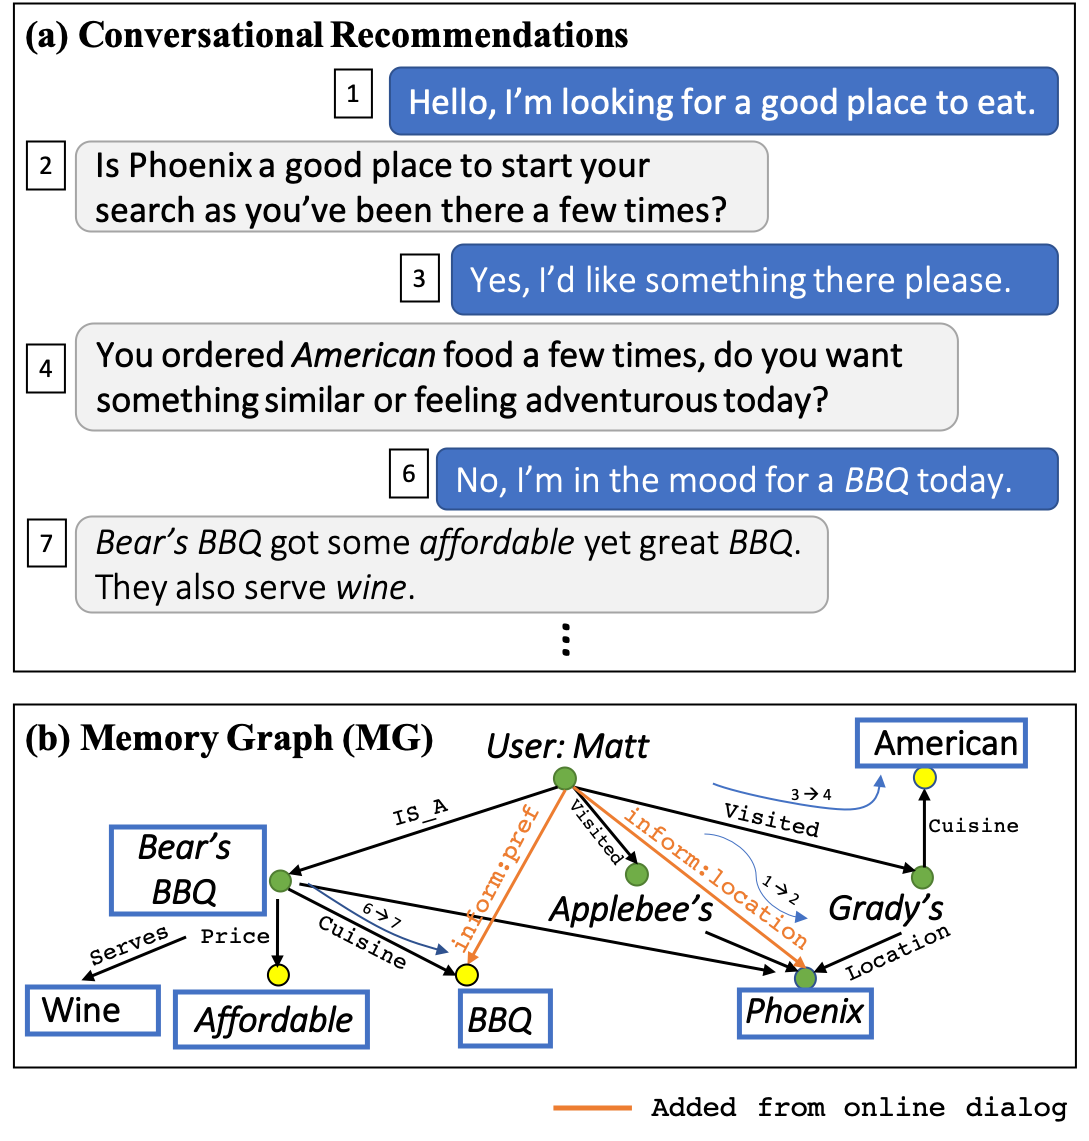
\includegraphics[width=0.9\columnwidth]{fig/acl19_teaser.png}
    %\caption{A conceptual illustration of \textbf{Memory-grounded conversational recommendation}. (1) Conversational recommendation allows users to express preferences and requirements through dialogs. (2) Our \textit{MGConvRex} corpus is grounded on the memory graph (MG), which represents user's past preferences as well as newly added preferences.}
    \caption{Conceptual illustration of Memory-grounded conversational recommendation}
\label{fig:dialog}
\vspace{-3mm}
\end{figure}

Conversational recommendation systems \cite{li2018towards} are recently introduced to mitigate some of these challenges by tracking users' up-to-date preferences through dialogs.
Most of the previous works focus on extending the conventional task-oriented dialog literature with a recommender system, which allows the conversational system to update user preferences online by asking relevant questions (called ``System Ask User Respond (SAUR)'' for the current dialog.

In summary, existing systems either favor a static offline recommendation over existing users or items or obtain short-term online updates on users' preferences via dialogs.
However, they unnaturally contrast offline with online preference learning and neglect the fact that the knowledge about a user is \textit{cumulative} in nature.
An intelligent system should be able to dynamically maintain and utilize knowledge about a user collected so far for recommendations.

To this end, we first introduce a novel concept called \textit{user memory graph} to represent dynamic knowledge about users and associated items in a structured graph (e.g., previous offline history of items visited/recommended, user preferences newly obtained through dialogs, etc.), allowing for easy and holistic reasoning for recommendations.
We then propose a new conversational recommendation system grounded onto this graph, conceptually defined more formally as follows:

\noindent\textbf{Memory-grounded Conversational Recommendation}:
Given the history of previous items $\mathcal{H}$ (interacted or visited, etc.), candidate items $\mathcal{C}$ for recommendation, and their attributes (values), 
an agent first (1) constructs a user memory graph $\mathcal{G} = \{(e, r, e')\vert e, e' \in \mathcal{E}, r \in \mathcal{R} \}$ for user $e_u$; 
then (2) for each turn $d \in D$ of a dialog, the agent updates $\mathcal{G}$ with tuples of preference $\mathcal{G}' \gets \mathcal{G} \cup \{(e_u, r_1, e_1), \dots\}$ ;
(3) performs reasoning over $\mathcal{G}'$ to yield a dialog policy $\pi$ that
either (i) performs more rounds of interaction by asking for more preference, 
or (ii) predicts optimal (or ground truth) items for recommendations $\mathcal{T} \subset \mathcal{C}$.

\textbf{Related Work}

\noindent \textbf{Conversational Recommendation}:
Much existing research on conversational recommendation focus on combining a recommender system with a dialog state tracking system, through the ``System Ask User Respond (SAUR)'' paradigm.
Once enough user preference is collected, such systems often make personalized recommendations to the user.
For instance, \cite{li2018towards} proposes to mitigate cold-start users by learning users' preferences during conversations and by linking the learned preferences to existing similar users in a traditional recommender system.

\cite{sun2018conversational,kang2019recommendation} propose a reinforcement learning (RL) setting for a conversational recommendation system, where the dialog policy is learned with multiple policies and recommendation signals.

\cite{zhang2018towards} leverages reviews to mimic online conversations to update an existing user's preference and re-rank items.

\noindent \textbf{Task-oriented Dialogue Systems} are widely studied with multiple popular benchmark datasets \cite{dstc2, woz, multiwoz, multiwoz2.1,sgd-dst}.
Most of the state-of-the-art approaches \cite{trade,bert-dst-alexa,bert-dst-cmu} focus on improving dialog state tracking with span-based pointer networks, which predicts information essential in completing a specified task (e.g., hotel booking, etc.)

Note that while conversational recommendation systems bears similarity to task-oriented dialog systems, the key difference is that conversational recommendation aims to collect user's fine-grained soft preferences or sentiments, and utilize them collectively for ranking of items or asking better questions (policy selection), instead of collecting hard constraints (e.g., number of people, time and location) to filter a database and locate a record. 

\noindent \textbf{Graph Reasoning}:
Graph network \cite{scarselli2008graph,duvenaud2015convolutional,defferrard2016convolutional,kipf2016semi} is a type of neural networks proposed to operate on graph structures. 
Several extensions to the original graph neural network have been proposed \cite{li2015gated,pham2017column},
most notably R-GCNs \cite{schlichtkrull2018modeling}, which can be applied on large-scale and highly multi-relational data.
Many applications of GNNs include \cite{Xian2019ReinforcementKG}, which introduces graph-based reasoning for an offline recommendation system.
A few works have recently been proposed to allow graph reasoning in dialog systems.
\cite{Moon+19a, Moon+19b} propose new corpus to learn knowledge graph paths that connect dialog turns.
\cite{tuan-etal-2019-dykgchat} introduces a knowledge-grounded dialog generation task given a knowledge graph that is dynamically updated.
However, these workes often focus on response generation and do not address the conversational recommendation task.


\textbf{Definition of Dialog Acts, SLots and Values}

\label{chap6:sec:form}
As discussed in the introduction, one key step to enable a dialog being grounded and maintained on a user memory graph is to first define the semantic space of dialog acts, items, their slots and values (we borrow these terms from task-oriented dialog system, which refer to items' attributes) for utterances from both the user and agent.
As a result, agents can turn unstructured utterances into structured data for user memory graph maintenance, integration and potentially future explainable reasoning for policy.
In this section, we first introduce the dialog acts for recommendation and then introduce slots and values specifically defined for the recommendation in a restaurant domain.

\textbf{Dialog Acts}
\label{chap6:sec:dialog_act}

The goal of designing dialog acts $\mathcal{A}$ is to formalize the intentions from both the user and agent sides. 
\ref{chap6:tbl:dialog_act} demonstrates the dialog acts for both the user and the agent.
From the agent's perspective, 
note that although existing conversational recommendation\cite{sun2018conversational,li2018towards,zhang2018towards} assumes a passive user interacts with the system and propose a System Ask – User Respond (SAUR) paradigm, we further allow the user to actively participate in the recommendation by allowing User Ask - System Respond (UASR) paradigm. In our dialog act, \textit{Open question}, \textit{Yes/no question} and \textit{Inform} can be used by a user to actively participate in the conversation. The dataset we created from crowd workers also indicates that human likes to use these active dialog acts in the context of conversational recommendation (see Appendix).


\begin{table}
    \centering
    \scalebox{0.65}{
        \begin{tabular}{l|l l}
        \hline
        \textbf{Dialog Act $a$} & \textbf{Description} & \textbf{Examples} \\
        \hline
        \textbf{User-side} & & \\
        \hline
        Greeting & Greeting to the agent & I'd like to find a place to eat. \\
        Inform & Actively inform the agent your preference & I'd like to find a \textit{thai} restaurant . \\
        Answer & Answer to a question from the agent & I prefer \textit{thai} food. \\
        Reply & Reply to a recommendation & I'll give it a try.\\
        Open question & Actively ask an open question about a recommended item. & What kind of food do they serve ? \\
        Yes/no question & Actively ask an yes/no question about a recommended item. & Do they serve \textit{thai} food ? \\
        Thanks & Thanks the agent & Thanks for your help. \\
        \hline
        \textbf{Agent-side} & & \\
        \hline
        Greeting & Greeting to the user. & How may I help you today ?\\
        Open question & Ask an open question about a slot to the user & What kind of food do you prefer ? \\
        Yes/no question & Ask a yes/no question about a value of a slot & I saw you've been to \textit{thai} restaurant, do you still like that ? \\
        Recommendation & Recommend items to the user. & How about \textit{burger king}, which serves \textit{fast food} ? \\
        Answer & Answers user's questions on an item. & They serve \textit{thai} food.\\
        Thanks & Thanks the user & Enjoy your meal. \\
        \hline
        \end{tabular}
    }
    \vspace{-2pt}
    %\caption{Dialogue acts for agent and user $\mathcal{A}$: the spans of items/slot values are italized.}     
    \caption{Dialog acts for agent and user $\mathcal{A}$}     
    \vspace{-11pt}
\label{chap6:tbl:dialog_act}
\end{table}

\textbf{Slots and Values}
\label{chap6:sec:slotvalue}

This paper focuses on the recommendation in the restaurant domain.
We utilize the customer review dataset, which is widely used in existing research in recommender systems.
By leveraging the metadata of restaurants, we define slots $\mathcal{S}$ and their values $\mathcal{V}$ as shown in \ref{chap6:tbl:dialog_slot}. 
We select $\vert \mathcal{S} \vert = 10$ popular slots with rich values that can be encountered in the restaurant domain.
We omit the full set of values for brevity and only list a few examples. (Please refer to our dataset for the exhaustive list).

\begin{table}[t]
    \centering
    \scalebox{0.7}{
        \begin{tabular}{l|l}
        \hline
        \textbf{Slot $e_s$} & \textbf{Example Value $e_v$} \\
        \hline
        location & Las Vegas, NV; Toronto, ON\\
        category & fast food; burger; thai\\
        price & cheap; expensive\\
        parking & garage; valet; lot\\
        noise & average; quiet\\
        ambience & classy; intimate\\
        alcohol & full bar; beer and wine \\
        good for meal & brunch; lunch; dinner\\
        wifi & paid; free\\
        attire & casual; formal\\
        \hline
        \end{tabular}
    }
    \vspace{-4pt}
    %\caption{Available slots $\mathcal{S}$ and example of their associated values $\mathcal{V}$.}     
    \caption{Slots $\mathcal{S}$ and values $\mathcal{V}$.}     
    \vspace{-10pt}
\label{chap6:tbl:dialog_slot}
\end{table}


\textbf{Dataset}
\label{chap6:sec:dataset}

Based on the definition in Chapter \ref{chap6:sec:form}, we create a large-scale dataset called \textit{MGConvRex}.
To the best of our knowledge, this is the first dataset for conversational recommendation that is grounded onto structured data of users' profile and items.
Although curating a dataset for a task-oriented dialog system may involve building artificial scenarios (a pre-defined setting for collecting a dialog) \cite{li2016user,li2018microsoft} due to limited access of real-world data for a particular task, conversational recommendation can leverage rich user behaviors that persist in the wild datasets of recommender system.  
As a result, we first introduce a simple way to create large-scale scenarios for dialog transcription, as in Chapter \ref{chap6:sec:scenario}.
Then we set up a Wizard-of-Oz environment \cite{dstc2,woz,multiwoz,multiwoz2.1} to collect dialogs from crowd workers and further annotate transcribed dialogs based on scenarios, as in Chapter \ref{chap6:sec:woz}.
Our \textit{MGConvRex} can be used for research in almost all crucial components of a dialog system such as natural language understanding, sentiment analysis, dialog state tracking, dialog policy generation, natural language generation, etc.

\textbf{Scenario Generation}
\label{chap6:sec:scenario}

A scenario is a pre-defined user-agent setting to collect a dialog between two crowd workers, where one plays the user and the other plays the agent.
Let $\mathbb{B}=\{0, 1\}$ be a binary number.
We define a scenario consisting of the following parts: $(e_u, C, H, V, P, \mathcal{T} )$, where $e_u$ is a user, $C \in \mathbb{B}^{\vert \mathcal{C} \vert \times \vert \mathcal{V} \vert}$ means the candidate items $\mathcal{C}$ and their associated values $\mathcal{V}$, $H \in \mathbb{B}^{\vert \mathcal{H} \vert \times \vert \mathcal{V} \vert}$ is about visited items $\mathcal{H}$ and their values user $e_u$ has been to and known to the agent, $V \in \mathbb{B}^{\vert \mathcal{V} \vert \times \vert \mathcal{S} \vert}$ indicates values with their associated slots, $P \in \mathbb{B}^{\vert \mathcal{S} \vert \times \vert \mathcal{V} \vert} $ is the user preference (which value the user prefer for a slot) and $\mathcal{T} \subset \mathcal{C}$ is the ground-truth items. 
Each scenario is constructed in the following way:
\begin{itemize}
\setlength\itemsep{0.1em}
    \item Preprocess reviews to keep users and items (restaurants) with at least 10 reviews (10-core users/items). 
    We further filter out users with more than 100 reviews as they are suspected to be spam reviewers (not real-world users).
    \item Sort items (of reviews) by time and use a pre-defined timestamp (e.g.,  01/01/2014) to separate items into two groups: visited items and future items for all users.
    \item For each user, random select $\vert \mathcal{T} \vert = 1$ \footnote{We use 1 ground-truth item to reduce the load of the transcribers and increase the difficulty of reasoning.} items (with 4 or 5 ratings) as the \textit{ground-truth items} $\mathcal{T}$. Use the slots / values of the ground-truth items as \textit{user preference} $P$.
    \item For each user, negatively sample $\vert \mathcal{C} \vert - \vert \mathcal{T} \vert $ items and combine them with the ground-truth items $\mathcal{T}$ as \textit{candidate items} $\mathcal{C}$ \footnote{We choose $\vert \mathcal{C} \vert \in [10, 20]$ candidate items.} from all available items\footnote{To allow real-world recommendation setting, we ensure certain similarity over candidate items such as all locations are from the same state as the ground-truth items.}.
    \item For each user $e_u$, create two scenarios: one with \textit{visited items} $\mathcal{H}$ and one without. We keep $\vert \mathcal{H} \vert \in [5, 20]$ visited items to ensure enough statistical information for a user's past history.
\end{itemize}

\begin{table*}
    \centering
    \scalebox{0.83}{
        \begin{tabular}{l|c|c|c||c|c|c|c}
        \hline
        \textbf{Dataset} & \multicolumn{3}{c||}{\textbf{All Dialogs}} &  \multicolumn{2}{c|}{\textbf{Dialogs w/ History }} & \multicolumn{2}{c}{\textbf{Dialogs w/o History}} \\
        \hline
         & \# of Dial. & \# of Turns & Avg. \# of Turns & \# of Dial. & Avg. \# of Turns & \# of Dial. & Avg. \# of Turns \\
        \hline
Train & 3225 & 30858 & 9.57 & 1570 & 9.52 & 1655 & 9.62 \\
Dev & 266 & 2488 & 9.35 & 137 & 9.18 & 129 & 9.53 \\
Test & 2078 & 19818 & 9.54 & 982 & 9.45 & 1096 & 9.61 \\
        \hline
        \end{tabular}
    }
    %\caption{\textbf{Statistics of the Dataset}: Dialogs w/ or w/o History indicates whether scenarios include visited items $\mathcal{H}$. }
    \caption{Statistics of MGConvRex Dataset}     
\label{chap6:tbl:dataset}
\end{table*}

\textbf{Wizard-of-Oz Collection}
\label{chap6:sec:woz}

We build a wizard-of-oz system to randomly pair two crowd workers to engage in a chat session, where each scenario is split into two parts:
$(P, \mathcal{T})$ for user and $(e_u, C, H, V)$ for the agent.
So in each session, the worker playing the user can see a user's preference $P$ and ground-truth items $\mathcal{T}$. 
The worker playing the agent can only see candidate items $C$ and the user's visited items $H$ (if a scenario contains that).
The user can tell the agent information from preference $P$ via utterance or check whether recommended items $e_i \in \mathcal{T}$ and reply to agent accordingly (they are not allowed to tell the ground-truth directly). 
The job of a worker playing the agent is trying to guess the ground-truth item $e_t \in \mathcal{T}$, based on the values of the available candidate items $C$, the current preference collected from the user via dialog, and optionally the user's visited items $H$.
As a result, the goal of a conversation is like a game between the user and the agent, where the agent needs to guess the user's current preference and find the ground-truth item.
The collected behavior from the agent side reflects human-level intelligence of reasoning over candidate items for recommendation.
After transcribing a dialog, we further ask the workers to rate the whole dialog and each other's work, where
dialogs with ratings lower than 4 are filtered out.
Lastly, we annotate dialog acts, items, slots, values and users' utterance-level and entity-level sentiment for each turn of dialogs.
The guidelines, screenshots of the Wizard-of-Oz UI can be found in the Appendix.

\noindent \textbf{Summary of \textbf{MGConvRex}}:
\label{sec:dataset_stat}
After annotation, we split the dialogs by their associated scenarios into training, development and test sets.
Note that we enforce all sets to have no overlapping on users so that the training cannot carry the knowledge from any particular user into testing.
The statistics of MGConvRex can be seen in \ref{chap6:tbl:dataset}.

\textbf{Experimental Framework}

While there exist many frameworks for task-oriented dialog systems \cite{li2016user,li2018microsoft,lee2019convlab} due to its popularity,
to the best of our knowledge, there's no existing framework for conversational recommendation.
Hence we first develop a new framework for training, offline and online evaluation of supervised (imitation) learning and reinforcement learning agents.
One key component of our framework is the rule-based user simulator, which can be served for both evaluation and training of reinforcement learning agent.

\textbf{Results}
\label{chap6:sec:exp}

\textbf{Evaluation Metrics}

We propose the following metrics to evaluate UMGR over the MGConvRex dataset both offline (against the collected dialogs) and online (against user simulator).

\textbf{Offline metrics}

We report the following metrics to evaluate the model's performance on dialog acts prediction, turn-level prediction over entities (items, slots, and values), and dialog-level item prediction.

\noindent \textbf{Act Accuracy \& F1} are reported for all dialog acts against turns in the testing set.

\noindent \textbf{Entity Matching Rate (EMR, k@1, 3, 5)} (Turn-level): these metrics measure the predicted top-$k$ entities against the annotated test dialogs. 
Note that the types of predicted entities (items, slots or values) depend on the predicted dialog acts $\hat{y}^\mathcal{A}$, so correctly predicted entities must have correctly predicted dialog acts first.

\noindent \textbf{Item Matching Rate (IMR)} (Dialog-level): this measures all predicted items in a dialog against the ground-truth item $e_t$.

\textbf{Online metrics}

In addition to offline evaluation, we report the following online metric against the user simulator to dynamically test the performance of recommendation. This mitigates an assumption in offline metrics that all past turns (from the human-annotated dialogs) are correct, which limits the interactive evaluation of conversations.

\noindent \textbf{Success Rate}: tracks whether the interaction with user simulators yields the ground-truth item $e_t$. We use the scenarios from the same test-set dialogs used for the offline evaluation. The maximum number of turns is simulated as 11.

\begin{table*}[!t]
    \centering
    \scalebox{0.83}{
        \begin{tabular}{l|l|l|l|l|l|l||c}
        \hline
\multirow{3}{*}{\textbf{Methods}} & \multicolumn{6}{c||}{\textbf{Offline Evaluation}} & \multicolumn{1}{c}{\textbf{Online Evaluation}} \\
\hline
& \textbf{Act Acc.}  & \textbf{Act F1} & \multicolumn{3}{c|}{\textbf{EMR}} & 
\textbf{IMR} & \textbf{Success Rate} \\
\hline
& & & @1 & @3 & @5 &  & \\
\hline
\hline
RandomAgent & 0.1769 & 0.182 & 0.0229 & 0.0229 & 0.0229 & 0.052 & 0.0659 \\
RecAgent      & 0.2568 & 0.0681 & 0.0262 & 0.0262 & 0.0262 & 0.3826 & 0.3855 \\
Pretrained Emb. & 0.2859 & 0.0741 & 0.1264 & 0.2484 & 0.316 & 0.0 & 0.0 \\
%UMGR & 0.61 & 0.5 & 0.22 & 0.38 & 0.44 & 0.33 & &  \\
\hline
%UMGR & Act Acc.  & Act F1 & \multicolumn{3}{c|}{EMR @1 @3 @5} & IMR & SuccessRate \\
\hline
UMGR (Proposed) & \textbf{0.643} & \textbf{0.5534} & 0.2329 & \textbf{0.4416} & \textbf{0.487} & 0.5226 & \textbf{0.4315} \\
- No Dialogue Acts & 0.3914 & 0.2137 & 0.2503 & 0.4383 & 0.4777 & 0.6165 & 0.4293 \\
- Prev. User Act Only & 0.6187 & 0.5375 & 0.2255 & 0.4175 & 0.4561 & 0.5693 & 0.4032 \\
- Static $\mathcal{G}$ & 0.6355 & 0.5452 & 0.0957 & 0.2769 & 0.3494 & 0.0914 & 0.11 \\
\hline
%UMGR on w/ or w/o His. & Act Acc.  & Act F1 & \multicolumn{3}{c|}{EMR @1 @3 @5} &  IMR & SuccessRate \\
\hline
UMGR w/ History & 0.5778 & 0.4761 & 0.0769 & 0.2111 & 0.2987 & 0.2872 & 0.2592 \\
UMGR w/o History & 0.6146 & 0.4575 & 0.0597 & 0.1546 & 0.2498 & 0.1122 & 0.1032 \\
        \hline
        \end{tabular}
    }
    \vspace{-2pt}
    %\caption{Results of both offline and online evaluation: EMR stands for entity matching rate, which compares all types of predicted entities against annotated ones when the dialog act is predicted correctly; IMR stands for item matching rate, which evaluates predicted items against the ground-truth item across all turns.}     
    \caption{Results of UMGR}     
    \vspace{-12pt}
\label{chap6:tbl:result}
\end{table*}

\textbf{Compared Methods}

Our framework implements the following methods:\\
\noindent \textbf{RandomAgent}: As a baseline, we implement an agent that randomly picks a dialog act and randomly pick a candidate item/slot/value to fill the current response to the user.\\
\noindent \textbf{RecAgent}: The agent always chooses \textit{Recommendation} as the dialog act to enact and select a random item that has not been tried from candidate items. This leads to sub-optimal performance as it does not use or collect user preferences.\\
\noindent \textbf{Pretrained Embeddings}: 
We pre-train the graph embeddings for all entities and relations from the MG across all scenarios in the training set using the TransE-based graph prediction approaches \cite{Nickel+15}.
We utilize these for prediction of the future item/slot/value without having the R-GCN layers.
While this approach is widely used in the related literature and carries cross-scenario knowledge, we show that using pre-trained graph embedding alone is sub-optimal for a particular user and that the dialog policy needs to perform dynamic reasoning over the user memory graph.\\
\noindent \textbf{UMGR} (\textbf{Proposed}): This is the proposed R-GCN based model. We choose the batch size to be 32, all hidden states to be size 64. The number of maximum dialog acts is set to 10. We use 5 layers of R-GCN based on validation on the development set. $\alpha, \beta, \gamma$ are set as 10, 10, 100 based on the scales of losses of different types, respectively. 
% \todo{check missing hyperparameters} 
We further conduct the following ablation studies.\\
\noindent \textbf{- No Dialog Acts}: this study removes the dialog acts encoder, demonstrating the importance of the dialog acts in policy generation.

\noindent \textbf{- Prev. User Act Only}: this study only uses the most recent dialog act from the user. We use this to show how many past dialog acts are needed for good policy generation.

\noindent \textbf{- Static $\mathcal{G}$}: uses the initial user memory graph without making any updates during the conversation. We use this study to demonstrate that dynamic update of the user memory graph is crucial for reasoning better dialog policy.\\

\noindent \textbf{- w/ History} v.s. \textbf{- w/o History}: analyzes the effect of the history of visited items $\mathcal{H}$ (the last two dataset folds in \ref{chap6:tbl:dataset}). We use these two baselines to demonstrate that prior knowledge of user memory history aids in predicting dialog policy.


\textbf{Result Analysis}

The results are shown in \ref{chap6:tbl:result}. From the results, we can see that UMGR achieves good performance for most of the metrics.
%\todo{we didn't talk about a rule-based agent I think it's fine. agreed} 

\noindent \textbf{UMGR} is effective in leveraging knowledge in the user memory graph.
While the UMGR model already achieves reasonable accuracy in dialog policy prediction relying just on the user memory graph (\textit{-No Dialogue Acts}),
adding previous dialog act from the user (\textit{- Prev. User Act Only}) significantly improves the performance.
%The competitive performance with (\textit{- Prev. User Act Only}) indicates that a good amount of user knowledge is contained in the user memory graph, without having to resort much to previous turns.
Lastly, we show that keeping user memory graph updated is crucial, as seen in \textit{static $\mathcal{G}$} not providing good rankings for entities.  

\noindent \textbf{UMGR vs. Pre-trained Graph Embeddings}. We confirm that the static pre-trained graph embeddings provide limited capacity for reasoning over a large-graph across multiple scenarios to learn user-specific dialog policy, leading to poor performance in the recommendation.

\noindent \textbf{w/ \textit{vs} w/o Hisory}. Lastly, the contrasting results for with and without visited items $\mathcal{H}$ in a user memory graph indicate that having more knowledge about a user's experience is important in conversational recommendation.

%\textbf{Conclusion}:
%We build a conversational recommendation system that can collect and maintain a user's up-to-date needs and preferences for the recommendation.
We release a novel dataset with \textit{user memory graph} grounding based on scenarios generated from the behaviors of real-world users.
The user memory graph has the benefits of both accumulating pieces of knowledge about a user and interpretability.
Experimental results on our R-GCN based reasoning model (UMGR) show promising results for dialog acts, items, slots, and values prediction.

\chapter{Conclusion}
The paradigm of lifelong learning is essential for learning beyond the classic deep learning approach.
Looking forward, the world keeps evolving and yields new data for new tasks, which probably are long-tailed or heavily-tailed.
The existing approach may represent the majority general features well and assume they are generally good for any new knowledge.
It lacks enough capability to represent the vast kinds of specific features that are required each (new) task.
To make the learning effective in the long-term, an AI agent must be able to adapt to the changes in the world.
This dissertation explores different forms of lifelong learning tasks, including classification, word embedding, contextualized word embedding, graph reasoning, and NLP applications.
However, the research of lifelong learning does not stop just at these formulations.
I expect future extended research of lifelong representation learning in the following areas: (1) similarity spaces of neural network that supports lifelong learning; (2) meta-learning over the formulation of lifelong learning tasks; (3) error-robust accumulation of knowledge.